
%%%%%%%%%%%%%%%%%%%%%%% file typeinst.tex %%%%%%%%%%%%%%%%%%%%%%%%%
%
% This is the LaTeX source for the instructions to authors using
% the LaTeX document class 'llncs.cls' for contributions to
% the Lecture Notes in Computer Sciences series.
% http://www.springer.com/lncs       Springer Heidelberg 2006/05/04
%
% It may be used as a template for your own input - copy it
% to a new file with a new name and use it as the basis
% for your article.
%
% NB: the document class 'llncs' has its own and detailed documentation, see
% ftp://ftp.springer.de/data/pubftp/pub/tex/latex/llncs/latex2e/llncsdoc.pdf
%
%%%%%%%%%%%%%%%%%%%%%%%%%%%%%%%%%%%%%%%%%%%%%%%%%%%%%%%%%%%%%%%%%%%


\documentclass[runningheads,a4paper]{llncs}
\usepackage{hyperref}
\usepackage{amsmath}
\usepackage{amsfonts}%,amsthm,
\usepackage{amssymb}

%\usepackage{amsthm}
\usepackage{dsfont}
\setcounter{tocdepth}{3}
\usepackage{graphicx}
\usepackage{subfigure} 
\usepackage{epstopdf}

% For algorithms
\usepackage{algorithm}
\usepackage{algorithmic}

\def\N{\mathbb{N}}
\def\Z{\mathbb{Z}}
\def\R{\mathbb{R}}
\def\C{\mathcal{C}}

\def\F{\mathcal{F}}
\def\G{\mathcal{G}}
\def\A{\mathcal{A}}
\def\M{\mathcal{M}}
\def\ICA{ICA$_{\mathcal{S\!N}}$}
\def\SN{\mbox{$\mathcal{S\!N}$}}
\DeclareMathOperator*{\argmin}{argmin}
\DeclareMathOperator*{\argmax}{argmax}

\def\x{\mathrm{x}}
\def\z{\mathrm{z}}
\def\m{\mathrm{m}}
\def\e{\varepsilon}
\def\d{\delta}
\def\w{\omega}
\def\v{\mathrm{V}}
\def\m{\mathrm{m}}

\def\F{\mathcal{F}}
\def\G{\mathcal{G}}
\def\S{\mathcal{S}}
\def\A{\mathcal{A}}

\def\KL{\mathrm{KL}}

\def\for{\mbox{  for }}
\def\mle{\mathrm{mle}}
\def\diag{\mathrm{diag}}
\def\cov{\mathrm{cov}}
\def\card{\mathrm{card}}
\def\aff{\mathrm{aff}}
\def\span{\mathrm{span}}
\def\nor{\mathcal{N}}

\def\ICA{ICA$_{\mathcal{S\!N}}$}
\def\1{\mathds{1}}
\def\X{\mathbf{X}}
\def\S{\mathbf{S}}


\newtheorem{observation}{Observation}[section]



\usepackage{url}
\urldef{\mailsa}\path|{przemyslaw.spurek,jacek.tabor}@ii.uj.edu.pl|
\urldef{\mailsb}\path|przemyslaw.rola@outlook.com|
\urldef{\mailsc}\path|{przemyslaw.spurek,jacek.tabor}@ii.uj.edu.pl|    
\urldef{\mailsd}\path|{aleksander.czechowski}@dynniq.com|
\newcommand{\keywords}[1]{\par\addvspace\baselineskip
\noindent\keywordname\enspace\ignorespaces#1}

\begin{document}

\mainmatter  % start of an individual contribution

% first the title is needed
\title{Non-square ICA based on the asymmetry}

% a short form should be given in case it is too long for the running head
\titlerunning{Lecture Notes in Computer Science+}

% the name(s) of the author(s) follow(s) next
%
% NB: Chinese authors should write their first names(s) in front of
% their surnames. This ensures that the names appear correctly in
% the running heads and the author index.
%
\author{P. Spurek%
%\thanks{...}%
\and J. Tabor \and P. Rola \and A. Czechowski}
%
%\authorrunning{Lecture Notes in Computer Science: Authors' Instructions}
% (feature abused for this document to repeat the title also on left hand pages)

% the affiliations are given next; don't give your e-mail address
% unless you accept that it will be published
\institute{Faculty of Mathematics and Computer Science, 
Jagiellonian University, 
\L ojasiewicza 6, 
30-348 Cracow, 
Poland\\
\mailsa\\
Department of Mathematics of the Cracow University of Economics, 
Rakowicka 27,
31-510 Cracow, 
Poland\\
\mailsb\\
Dynniq B.V.,
Basicweg 16,
3821 BR Amersfoort,
The Netherlands
\mailsd
%\mailsc\\
%\url{http://www.springer.com/lncs}
}
%\author{P. Rola}
%
% NB: a more complex sample for affiliations and the mapping to the
% corresponding authors can be found in the file "llncs.dem"
% (search for the string "\mainmatter" where a contribution starts).
% "llncs.dem" accompanies the document class "llncs.cls".
%

\toctitle{Lecture Notes in Computer Science}
\tocauthor{Authors' Instructions}
\maketitle


\begin{abstract}
In its basic form Independent Component Analysis (ICA) aims to find an invertible linear transformation so that the transformed data has independent components. In the case when number of sources is less than the number of sensors, the task has an additional step which consists of filtering the possible noise - in such situation we are looking for so-called non-square mixing matrix.
 
 
Due to computational constraints, principal component analysis is often used for dimension reduction prior to ICA (PCA+ICA). However, such approach commonly removes important information. In this paper we present a method based on split-gaussians \textbf{mozna pisac split-gaussians? troche nieformalnie, moze split-gaussian distributions?} which is dedicated for determining \textbf{a} non-square mixing matrix in ICA maximum likelihood framework.
The main idea is based on separation of components which are as not-normal \textbf{not-normal brzmi dziwnie ale moze to tylko ja? as far from normal as possible?} as possible\textbf{przecinek} from the noise, which is assumed to be gaussian. Experiments show that our method obtains better or comparable \textbf{comparable or better} results to most state-of-the-art ICA approaches.
\emph{abstract}\textbf{ usunac}
\keywords{ICA, PCA, Source separation}
\end{abstract}


%%%%%%%%%%%%%%%%%%%%%%%%%%%%%%%%
%%%%%%%%%%%%%%%%%%%%%%%%%%%%%%%%
\section{Introduction}
\label{introduction}
%%%%%%%%%%%%%%%%%%%%%%%%%%%%%%%%

Independent component analysis (ICA) is similar in many aspects to principal component analysis (PCA). In PCA we look for an orthonormal base in which the data components are not
linearly dependent (uncorrelated), while in 
ICA we search for the coordinate system in which the components are independent. More precisely the aim of ICA is to transform the observed data $\X$ into maximally independent components $\S$ with use of an invertible linear transformation $W$, called the {\em transformation matrix}: $$
\S = W^T \X.
$$

Popular ICA methodology does not directly attempt to find components that are independent but rather components that are as non-Gaussian as possible.
This follows from the fact that one of the theoretical foundations of ICA is given by the dual view at the Central Limit Theorem \cite{hyvarinen2000independent}, which states that the distribution of the sum (average or linear combination) of $N$ independent random variables approaches Gaussian as  $N\rightarrow \infty$. Obviously if all source variables are Gaussian, the ICA method will not work. 

Another common approach to ICA based on the maximum likelihood estimation~\cite{pham1997blind} is recently gaining popularity \cite{hyvarinen2004independent,samworth2012independent,ICA2017pattern}.  Then we search for the optimally fitted to data cordinate system $B$ and marginal
densities $f_i$ such that the data density factors in base $B$ as the product of maringal densities. To obtain an efficient method and avoid 
overfitting we have to restrict the marginal densities $f_i$ to a class $\F$ of densities which has not too many parameters which can be easily estimated (clearly from obvious reasons this class has to be different from gaussians).  As $\F$ we typically choose the super-Gaussian logistic density or other heavy tails distributions.

In many applications of ICA we deal with the case when several sensors measure the latents variables and the rest of them record only the noise. This happens when the number of sources is unknown and may be less than the number of sensors (then we are looking for so-called {\em non-square mixing matrix} $W$).
Such a case is common for example in the identification of brain networks
in functional  magnetic resonance imaging (fMRI) 
\cite{beckmann2012modelling,green2002pca}.
%and then we are looking for so-called non-square mixing matrix.
In practice, most approaches deal with this problem by first applying PCA to the observations prior to classic ICA (PCA+ICA) to meet the assumption of square mixing and to reduce computational costs \cite{hyvarinen2004independent}. Although numerically effective, this approach may fail as it is not invariant with respect to linear transformation, since PCA will find a ``noise'' component if
it is sufficiently large. 

%\begin{landscape}
\begin{figure*}[t]
% ensure that we have normalsize text
\normalsize
\begin{center}
\subfigure[Original images 42049 and 220075.] {\label{fig:image_ICA_int_1}
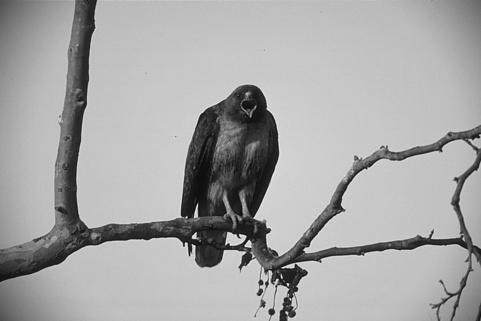
\includegraphics[width=1.6in]{2/2_6_or_1} 
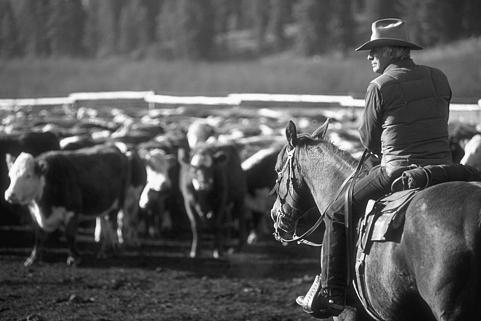
\includegraphics[width=1.6in]{2/2_6_or_2}
}
%%%%%%%%%%%%%%%%%%%%
%\subfigure[Sum and subtraction of images.] {\label{fig:image_ICA_int_2}
%\includegraphics[width=1.2in]{2/2_6_sum} 
%\includegraphics[width=1.2in]{2/2_6_div}
%} \\

%%%%%%%%%%%%%%%%%%%%
\subfigure[\ICA.] {\label{fig:image_ICA_int_3}
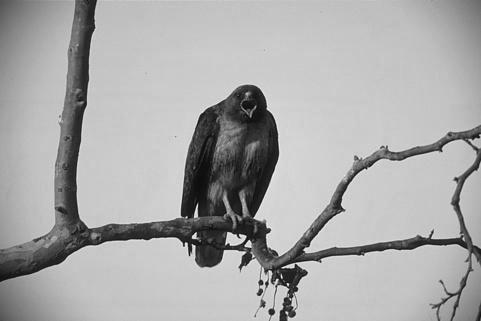
\includegraphics[width=1.6in]{2/2_6_ICA_FEW_II_2} 
}
\subfigure[FastICA.] {\label{fig:image_ICA_int_4}
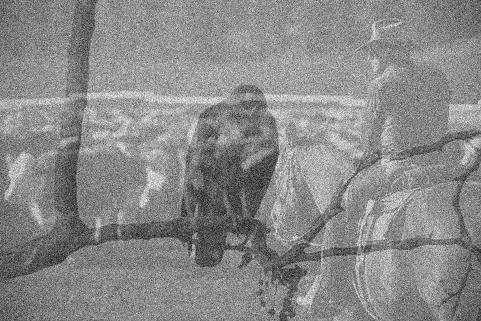
\includegraphics[width=1.6in]{2/2_6_ICA11_2} 
}
\subfigure[ProDenICA.] {\label{fig:image_ICA_int_5}
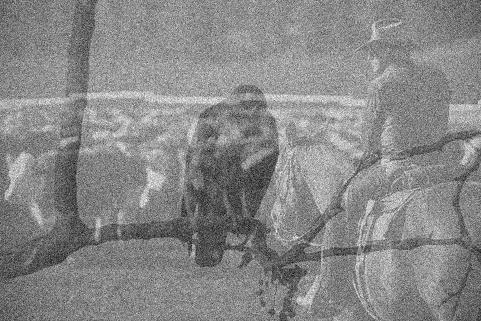
\includegraphics[width=1.6in]{2/2_6_ICA5_2} 
}\\
%%%%%%%%%%%%%%%%%%%%
\subfigure[\ICA.] {\label{fig:image_ICA_int_6}
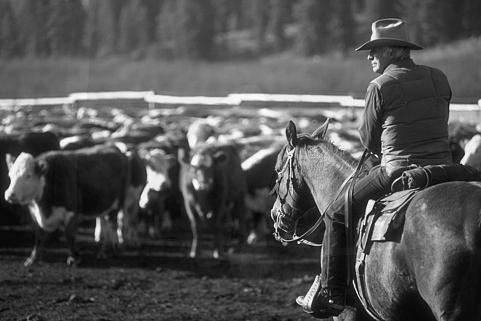
\includegraphics[width=1.6in]{2/2_6_ICA_FEW_II_1}
}
\subfigure[FastICA.] {\label{fig:image_ICA_int_7}
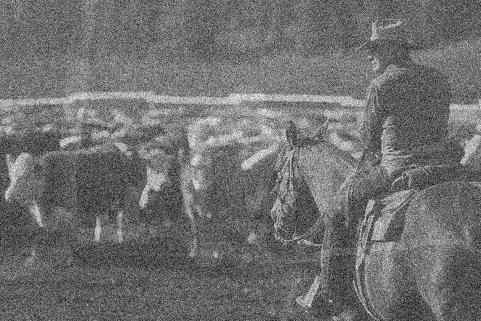
\includegraphics[width=1.6in]{2/2_6_ICA11_1}
}
\subfigure[ProDenICA.] {\label{fig:image_ICA_int_8}
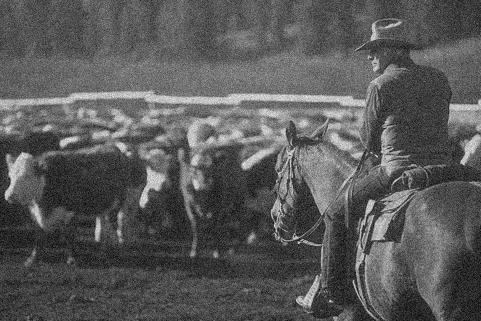
\includegraphics[width=1.6in]{2/2_6_ICA5_1}
}
\end{center}
\caption{Comparison of images separation by our method (\ICA), with FastICA and ProDenICA. Before mixing by a linear matrix, we added to the first two components given in (a) the third component given by random
normal noise. As we see \ICA{} was able to perfectly recover the two first components.}
\label{fig:image_ICA_int}
\end{figure*}

The aim of this paper is to propose a new density based approach to deal with this case which does not have the above
mentioned disadvantage. Our idea is to join the two earlier mentioned approaches to solving ICA - one based on the search for non-gaussian components and the
other based on density estimation - to deal with the case when the number of sources is smaller then that of sensors.  
Observe that the noise typically occurs as a sum of many independent
factors, and consequently thanks to the central limit theorem it typically has approximately gaussian distribution. This is why
one typically makes the assumption \cite{cover2012elements} that
$$
\text{\em noise components are comming from a gaussian noise.}
$$ 
Following the density approach to filter them out we fit the first $d$-components from a class of $\F$ of densities which is broader then gaussians, while the rest from the gaussians $\nor$ (the final choice of the value of parameter $d \in \{1,\ldots,D\}$ can be decided by applying either AIC or BIC criterion). Following \cite{ICA2017pattern} as $\F$ we take the class \SN{} of split-normal densities.

Our experiments show, which is illustrated by Figure \ref{fig:image_ICA_int}, that \ICA{} works as desired and effectively removes the components which contains gaussian noise. However, we cannot objectively conclude that it is better as compared to other state-of-the-art approaches, since the experiment 
was conducted in the setting optimal to our method as we assumed
that the noise was gaussian.

%%%%%%%%%%%%%%%%%%%%%%%%%%%%%%%%

%%%%%%%%%%%%%%%%%%%%%%%%%%%%%%%%
%%%%%%%%%%%%%%%%%%%%%%%%%%%%%%%%
\section{Related works}
\label{related_works}
%%%%%%%%%%%%%%%%%%%%%%%%%%%%%%%%

In literature exist a few approaches dedicated for non-square ICA problem.
Most of such method are dedicated for individual methods.
Attias and Schreiner \cite{attias1997blind} derived a likelihood based algorithm for separation of general sequences with a frequency domain implementation.
Belouchrani and Cardoso \cite{belouchrani1995maximum} presented a general likelihood approach allowing
for additive noise and for non-square mixing matrices. They applied the
method to separation of sources taking discrete values and estimated the
mixing matrix using an Expectation-Maximization (EM) approach with both a deterministic and a stochastic formulation. In \cite{moulines1997maximum} authors used the EM approach
for separation of autocorrelated sequences in presence of noise and explored
a family of flexible source signal priors based on Gaussian Mixtures. 

The assumption is that of square mixing is mostly unrealistic in  the case of EEG ant FMRI where the number of sources is less than the number of electrodes \cite{beckmann2004probabilistic,samarov2004nonparametric,shi2017investigating}. Therefore, many of algorithms dedicated for this task use a probabilistic ICA \cite{tipping1999probabilistic}.
The noisy ICA model can be approximated using a variant of PCA+ICA \cite{beckmann2004probabilistic}, where probabilistic PCA is used to estimate the number of components and achieve dimension reduction \cite{tipping1999probabilistic}.
In \cite{allassonniere2012stochastic} authors developed stochastic EM algorithms to estimate the noisy model and proposed parametric methods.

Other methods exploring non-Gaussian structure in multivariate data include non-Gaussian component analysis (NGCA) and projection pursuit \cite{blanchard2006search,kawanabe2007new}.
NGCA is a more general case of linear non-Gaussian component analysis (LNGCA) \cite{risk2015likelihood}
that allows non-linear dependence between the non-Gaussian components.

In the paper  \cite{miettinen2014deflation} authors propose a novel adaptive twostage deflation-based FastICA algorithm that allows one to use different nonlinearities for different components and optimizes the order in which the components are extracted.








%%%%%%%%%%%%%%%%%%%%%%%%%%%%%%%%
  
 %%%%%%%%%%%%%%%%%%%%%%%%%%%%%%%%
%%%%%%%%%%%%%%%%%%%%%%%%%%%%%%%%
\section{Theoretical foundations of \ICA{}}
\label{p}

In this section we present \textbf{the} theoretical foundations of the method.
We begin with the statement of the problem, next we focus our attention on the presentation of \textbf{zamiast tego wszystkiego, next we present} the class of densities we discuss \textbf{used zamiast we discuss}. Last \textbf{przecinek} we show \textbf{compute zamiast show} the gradient of the method \textbf{przecinek} which is needed in the optimization procedure.


\subsection{Statement of the problem}

Since this general \textbf{the zamiast this general} idea of the search for ICA \textbf{for independent components zamiast for ICA} with the use of
maximum likelihood is essential in our further considerations, for the convenience of the reader we first describe it briefly.
Assume that the random vector $\X$ in $\R^D$ has the density function $F(\x)$.
Suppose that the components of $\X$ are not independent, but that
we know (or suspect) that \textbf{moze usunac we know or suspect that?} there is a basis $B$ (we put $W^T=B^{-1}$) such that in that base the
components of $\X$ become independent. Observe \textbf{przecinek} that where \textbf{then zamiast where} $\w_i^T\x$ is the $i$-th coefficient of $\x$ in the basis $B$ ($\w_i$ denotes the $i$-th column of $W$), and therefore there exist densities 
$f_1,\ldots,f_D$ such that
\begin{equation} \label{eq:gen}
F(\x)=\det(W) \cdot f_1(\w_1^T\x) \cdot \ldots \cdot f_d(\w_d^T\x).
\end{equation}
Given $W$ and densities $(f_i)_{i=1}^D$ we introduce notation to represent
RHS \textbf{we denote the right-hand side} of the above equation \textbf{as follows}:
$$
F_W(f_1,\ldots,f_D)(\x)=\det(W) \cdot f_1(\w_1^T\x) \cdot \ldots \cdot f_d(\w_d^T\x).
$$
Thus we may \textbf{Let us now zamiast Thus we may} state the density based formulation of ICA in the case we have only a sample
$X$ from random vector $\X$.

\medskip

\noindent \textbf{THE?} GENERAL ICA PROBLEM (\textbf{the} maximum likelihood formulation). \\{\em Find densities $f_i$ and matrix $W$, so that $F$ given by
\eqref{eq:gen} optimally fits the data $X=(\x_i)$ with respect to the likelihood, that is that the value
$$
\sum_i \log F_W(f_1,\ldots,f_D)(\x_i)
$$
is maximized.
}

\medskip

Since the search over the space of all densities is not feasible, and could lead to overfitting, we naturally have to reduce to a subclass of all densities on $\R$ parametrized by a finite amount of parameters. Clearly, since 
ICA does not work if the data are gaussian, we have to choose a family $\F$ of densities which is distant from Gaussian ones. 

\medskip

\noindent ICA FOR DENSITY CLASS $\F$.\\ {\em Find \textbf{a} matrix $W$ and
densities
$
f_1,\ldots,f_D \in \F, 
$
such that the value of 
$$
\sum_i \log F_W(f_1,\ldots,f_D)(\x_i)
$$
is maximized.
}

\medskip

Similarly to \cite{ICA2017pattern} as a class \textbf{usun a class} $\F$ we are going to
take the class of split-gaussians, as 
as it is easy to deal with (small number of parameters) and is resistant to outliers\footnote{The reason is that split gaussians \textbf{moze split gaussian distributions}, instead at fitting the distribution with respect to heavy tails, fits the asymmetry of the data. \textbf{troche to zdanie ciezkie. Moze po prostu split gaussians are fitting well to asymmetrical data?}}.

As mentioned in the introduction, we assume that components which we would like to filter-out, \textbf{tu bez przecinka} are coming from a gaussian noise, and the \textbf{then zamiast the} aim it to fit the first $d$-components from a larger class of densities, while the rest from the gaussians $\nor$.\textbf{Poprzednie zdanie jest troche niezrozumiale, przepisz prosze (moze rozbij na dwa).} Thus our final problem can be stated as follows.

\medskip

\noindent ICA FOR DENSITY CLASS $\F$ WITH $d$ SOURCES. \\{\em Find \textbf{a} matrix $W$, densities 
$
f_1,\ldots,f_d \in \F \text{ and normal densities } f_{d+1},\ldots,f_D \in \nor,
$
so that the value of 
$$
\sum_i \ln F_W(f_1,\ldots,f_D)(\x_i)
$$
is maximized.
}

\medskip

Observe that the solution to the above problem is linearly invariant, that is if
$W$ is optimal for $X$ an $A$ is linear, then $W_A$ is optimal for $AX$,
where $W_A=(A^{-1})^TW$.

The continuous version of the condition we maximize in the case we know the density $f$
of the random variable $\X$ limits to
$$
\begin{array}{l}
\int \ln F_W(f_1,\ldots,f_D)(\x)f(\x) d\x %\\[1ex]
=-H(f,F_W(f_1,\ldots,f_D)),
\end{array}
$$
where the cross entropy $H(f,g)$ is given by the sum of entropy $H(f)$
and Kullback-Leibler divergence $D_{KL}(f,g)$. Thus the continuous version of the ICA problem
with $d$ sources reduces to the minimization of 
$$
D_{KL}(f,F_W(f_1,\ldots,f_D))
$$
over all matrices $W$ and densities $f_1,\ldots,f_D \in \F$. Since for fixed $f$ Kullback-Leibler divergence is minimized for $g=f$, we arrive at the following result, which says that in the ideal case 
by the discussed approach we restore the unmixing matrix if it exists.

\begin{theorem}
  Let $F$ be a density such that there exist \textbf{a} matrix $\overline W$ and densities
$$
\hat f_1,\ldots,\hat f_d \in \F \text{ and } \hat f_{d+1},\ldots,\hat f_D \in \nor
$$
such that 
$$
F=F_{\overline W}(\hat f_1,\ldots,\hat f_D).
$$
Then
$$
\begin{array}{l}
\overline W,\hat f_1,\ldots,\hat f_D %\\[1ex]
\begin{array}{l}
=\argmin \{F_{W}(f_1,\ldots,f_D): %\\[1ex] 
%\phantom{=\argmin \{}
W, f_1,\ldots,\bar f_d \in \F,f_{d+1},\ldots,f_D \in \nor
\}.
\end{array}
\end{array}
$$
\end{theorem}

\subsection{Split normal distribution}


In this section we discuss the class $\F$ we will use in our final algorithm of \ICA{}. The density of \SN{}, the one-dimensional split normal distribution \cite{villani2006multivariate}, is given by the formula
$$
\SN(x;m,\sigma^2,\tau^2) = \left\{ \begin{array}{l}
c \cdot \exp[-\frac{1}{2\sigma^2}(x-m)^2], \textrm{$x\leq m$}\\
c \cdot \exp[-\frac{1}{2\tau^2\sigma^2}(x-m)^2], \textrm{$x>m$}\\
\end{array} \right. \!\!\!\!,
$$
where $c=\sqrt{\frac{2}{\pi}}\sigma^{-1}(1+\tau)^{-1}$. 


As we see \textbf{przecinek} the split normal distribution comes from merging two opposite halves of two normal distributions in their common mode. The main advantage of \textbf{in using zamiast of} split normal distributions over normal one \textbf{moze over regular ones?} is that it \textbf{they zamiast it} allows \textbf{allow zamiast allows} data asymmetry. In 1982 John \cite{john1982three} showed \textbf{Moze It was shown by John.. i bez pisania roku} that the likelihood function can be expressed in a  form in which the scale parameters $\sigma$ and $\tau$ are an explicit function of the location parameter $m$.
In the case when $\F=\SN$
the density class considered in the previous subsection is given in the
explicit form by the following observation.

\begin{observation}\label{def:GSN}
  \textbf{Czemu Observation 31? Przenumeruj to jakos} A density of the multivariate split normal $d$ and normal $D-d$ distribution is given by
$$
\begin{array}{l}
\SN_{d}\nor_{D-d}(\x; \m,W, \sigma^2,\tau^2)=\\[6pt]
\det(W) \prod \limits_{j=1}^{d} \SN(\w_j^T(\x-\m);0,\sigma_j^2,\tau_j^2)%\cdot\\[1ex]
\cdot \prod \limits_{j=d+1}^{D} \nor(\w_j^T(\x-\m);0,\sigma_j^2),
\end{array}
$$
where $\w_{j}$ is the $j$-th column of non-singular matrix $W$, $\m = (m_1, \ldots, m_d)^T$, $\sigma = (\sigma_{1},\ldots,\sigma_{d})$ and $\tau=(\tau_{1},\ldots,\tau_{D-d})$.
\end{observation}

Observe that the above density probability function has mode in $\m$.
As a consequence of result of John \cite{john1982three} we can maximize the likelihood of the above function on data $X$ with respect to $\sigma$ and $\tau$.

\begin{theorem}\label{the:min}
Let $\x_1,\ldots,\x_n$ be given, and let $\m \in \R^D$ and matrix $W$
be fixed.  
Then the likelihood maximized w.r.t. $\sigma$ and $\tau$ is
\begin{equation}\label{eq:1}
\begin{array}{l}
 \hat{L}(X;\m,W) =   \frac{ 2^{(d-D/2)n} n^{dn/2} }{(\pi e)^{Dn/2}} %\cdot \\[1ex]
 \bigg( \frac{1}{|\det(W)|^{\frac{2}{3}}} \prod\limits_{j=1}^{d} g_{j}(\m,W) \bigg)^{-3n/2} 
\bigg( \prod\limits_{j=d+1}^{D} \frac{(s_1+s_2)}{n} \bigg)^{-n/2},
\end{array}
\end{equation}
where
$$
\begin{array}{c}
{g}_{j}(\m,W) = {s}_{1j}^{1/3} + {s}_{2j}^{1/3},
\\[1ex]
{s}_{1j}= \! \sum\limits_{i \in I_j}[ \w_{j}^T (\x_i-\m)]^2,  {I}_j=\{ i  \colon \w_{j}^T (\x_i-\m) \leq 0 \},
\\[1ex]
{s}_{2j}= \! \sum\limits_{i \in I_j^c}[ \w_{j}^T (\x_i-\m)]^2, {I}_j^c=\{ i \colon  \w_{j}^T (\x_i-\m) > 0 \},
\end{array}
$$
and the maximum likelihood estimators of $\sigma_{j}^2$ and $\tau_{j}$ are
\begin{equation}\label{eq:est}
\begin{array}{l}
\hat \tau_{j}(\m,W)=\left(\frac{s_{2j}}{s_{1j}}\right)^{1/3}, \qquad 1 \leq j \leq d\\[6px]
\hat \sigma_j^2(\m,W) = \left\{ \begin{array}{l}
\tfrac{1}{n} s_{1j}^{2/3} g_{j}(\m,W), \; 1 \leq j \leq d\\
\tfrac{1}{n} (s_{1j}+s_{2j}), \qquad d < j \leq D\\
\end{array} \right. \!\!\!\!.
\end{array}
\end{equation}
\end{theorem}
%\comment{Przemek R.- task 3. sprawdzic dowod Theorem \ref{the:min}}

\begin{proof}
See Section \ref{a1} (Appendix A).
\end{proof}

Thanks to the above theorem we can reduce the search for the maximum of the log-likelihood function for two parameters $\m \in \R^d$ and $W \in \M(\R^d)$.

\begin{equation}\label{equ:ll}
{l}(X;\m,W) = \frac{1}{|\det(W)|^{\frac{2}{3}}} \prod_{j=1}^{d} {g}_{j}(\m,W) \prod_{j=d+1}^{D} (s_{1j} + s_{2j})^{\frac{1}{3}}
\end{equation}
where $w_{j}$ stands for the $j$-th column of matrix $W$. 
Consequently, maximization of likelihood function is equivalent to minimization of  $\ln l$.

\begin{corollary}\label{c2}
Let $X \subset \R^d$, $\m \in \R^d$, $W \in \M(\R^d)$ be given, then
$$
\argmax_{\m,W} \hat{L}(X;\m,W) =  \argmin_{\m,W} \ln {l}(X;\m,W).
$$
\end{corollary}

%\subsection{Optimization}

To minimize $\ln l$ with the use classical gradient descent method \textbf{moze standard gradient methods? We wtyczce uzywamy BFGSa na przyklad to jakas wariacja gradient descentu},  we need
the formula for $\nabla \ln l$ (\textbf{the} gradient of the cost function). 

%Now we are ready to calculate gradient of our cost function.

%\begin{theorem}\label{ther:grad}
%Let $X \subset \R^d$, $\m = (\m_1, \ldots, \m_d)^T \in \R^d$, $W = (\w_{ij})_{1 \leq i,j \leq d}$ non-singular be given. 
%Then
%$\nabla_{\m}  \ln {l}(X;\m,W) = \left(  \frac{\partial \ln {l}(X;\m,W)}{\partial \m_1}, \ldots, \frac{\partial \ln {l}(X;\m,W)}{\partial \m_d} \right)^T$,
%where
%$$
%\begin{array}{l}
%\frac{\partial \ln {l}(X;\m,W)}{\partial \m_k} =
%\end{array}
%$$
%Moreover,
%$
%\nabla_{W} \ln {l}(X;\m,W) = \left[ \frac{\partial \ln \tilde{l}(X;\m,W)}{\partial \w_{pk}}  \right]_{1 \leq p,k \leq d},
%$
%where
%$$
%\begin{array}{l}
%\frac{\partial \ln \tilde{l}(X;\m,W)}{\partial \w_{pk}}  = .
%\end{array}
%$$
%and
%$$
%\begin{array}{c}
%%{g}_{j}(\m,W) = {s}_{1j}^{1/3} + {s}_{2j}^{1/3},
%%\\[1ex]
%{s}_{1j}= \! \sum\limits_{i \in I_j}[ \w_{j}^T (\x_i-\m)]^2, {I}_j=\{ i  \colon \w_{j}^T (\x_i-\m) \leq 0 \},
%\\[1ex]
%{s}_{2j}= \! \sum\limits_{i \in I_j^c}[ \w_{j}^T (\x_i-\m)]^2,  {I}_j^c=\{ i  \colon  \w_{j}^T (\x_i-\m) > 0 \}.
%\end{array}
%$$
%\end{theorem}

\begin{theorem}\label{ther:grad}
Let $X \subset \R^d$, $\m = (\m_1, \ldots, \m_d)^T \in \R^d$, $W = (\w_{ij})_{1 \leq i,j \leq d}$ non-singular be given. 
Then
$\nabla_{\m}  \ln {l}(X;\m,W) = \left(  \frac{\partial \ln {l}(X;\m,W)}{\partial \m_1}, \ldots, \frac{\partial \ln {l}(X;\m,W)}{\partial \m_d} \right)^T$,
where
$$
\begin{array}{l}
\frac{\partial \ln {l(X;\m,W)}}{\partial \m_k} =\sum\limits_{j=1}^d \frac{-2}{3({s}_{1j}^{\frac{1}{3}} + {s}_{2j}^{\frac{1}{3}})} \bigg(
\frac{1}{{s}_{1j}^{\frac{2}{3}}} \sum\limits_{i \in I_j} \w_j^T (\x_i - \m)  \w_{jk} +% \\[6pt]
\frac{1}{{s}_{2j}^{\frac{2}{3}}} \sum\limits_{i \in I_j^c} \w_j^T (\x_i - \m) \w_{jk}
\bigg)+ \\[6pt]
\sum\limits_{j=d+1}^D \frac{-2}{3(s_{1j}+s_{2j})} \cdot %\\[6pt]
\bigg(
 \sum\limits_{i \in I_j} \w_j^T (\x_i - \m)  \w_{jk} + %\\[6pt]
 \sum\limits_{i \in I_j^c} \w_j^T (\x_i - \m) \w_{jk}
\bigg).
\end{array}
$$
Moreover,
$
\nabla_{W} \ln {l}(X;\m,W) = \left[ \frac{\partial \ln \tilde{l}(X;\m,W)}{\partial \w_{pk}}  \right]_{1 \leq p,k \leq d},
$
where
$$
\begin{array}{l}
\frac{\partial \ln {l(X;\m,W)}}{\partial \w_{pk}} = -\frac{2}{3} (\w^{-1})^T_{pk} +\\[6pt]
 \frac{2}{3({s}_{1p}^{\frac{1}{3}} +{s}_{2p}^{\frac{1}{3}})} 
 \bigg(
{s}_{1p}^{-\frac{2}{3}} \sum\limits_{ i \in {I}_p} \w^T_p (\x_i - \m) (\x_{ik} - \m_k)
+ {s}_{2p}^{-\frac{2}{3}} \sum\limits_{ i \in {I}_p^c} \w^T_p (\x_i - \m) (\x_{ik} - \m_k) \bigg)+ \\[6pt]
\frac{2}{ 3(s_{1p}+s_{2p}) } \bigg( 
\sum\limits_{ i \in {I}_p} \w^T_p (\x_i - \m) (\x_{ik} - \m_k) + \sum\limits_{ i \in {I}_p^c} \w^T_p (\x_i - \m) (\x_{ik} - \m_k) \bigg),
\end{array}
$$
and
$$
\begin{array}{c}
%{g}_{j}(\m,W) = {s}_{1j}^{1/3} + {s}_{2j}^{1/3},
%\\[1ex]
{s}_{1j}= \! \sum\limits_{i \in I_j}[ \w_{j}^T (\x_i-\m)]^2, {I}_j=\{ 1 \leq i \leq n \colon \w_{j}^T (\x_i-\m) \leq 0 \},
\\[1ex]
{s}_{2j}= \! \sum\limits_{i \in I_j^c}[ \w_{j}^T (\x_i-\m)]^2,  {I}_j^c=\{ 1 \leq i \leq n \colon  \w_{j}^T (\x_i-\m) > 0 \}.
\end{array}
$$
\end{theorem}

\begin{proof}
See Section \ref{a2} (Appendix B).
\end{proof}


Thanks to the above Theorem we are able to use in our experiments the gradient descent for finding the minimum of our cost function.



%%%%%%%%%%%%%%%%%%%%%%%%%%%%%%%%

%%%%%%%%%%%%%%%%%%%%%%%%%%%%%%%%%%%%%%%%%%%%%%%%%%%%%%%%%%%%%%%%
%%%%%%%%%%%%%%%%%%%%%%%%%%%%%%%%
\section{Experiments}
\label{experiments}

%\begin{landscape}
\begin{figure*}[t]
% ensure that we have normalsize text
\normalsize
\begin{center}
\subfigure[Results of ICA methods in the case of mixture of images and Gaussian noise.] {\label{fig:rank1_a}
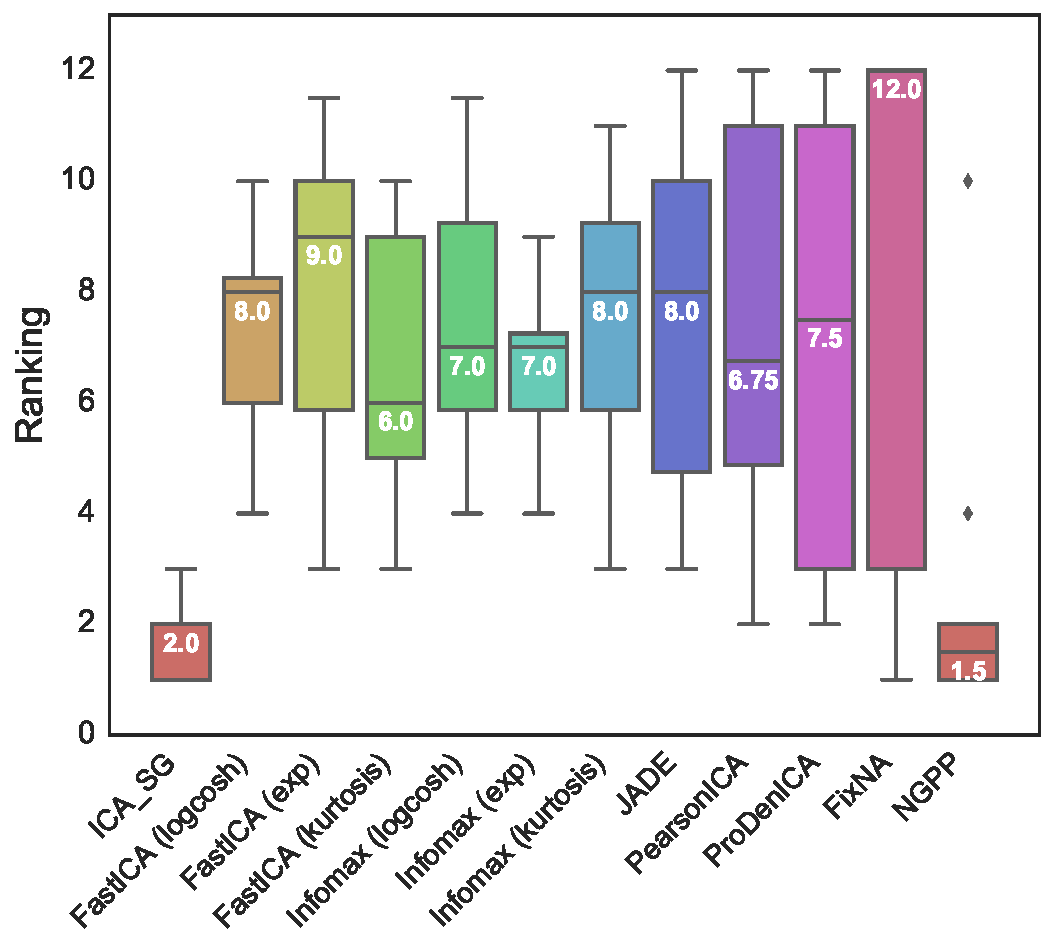
\includegraphics[width=2.2in]{ranking/images_boxplot-r1.pdf}
} \quad
\subfigure[Results of ICA methods in the case of mixture of images and salt and pepper \textbf{``salt and pepper''} noise.] {\label{fig:rank1_b}
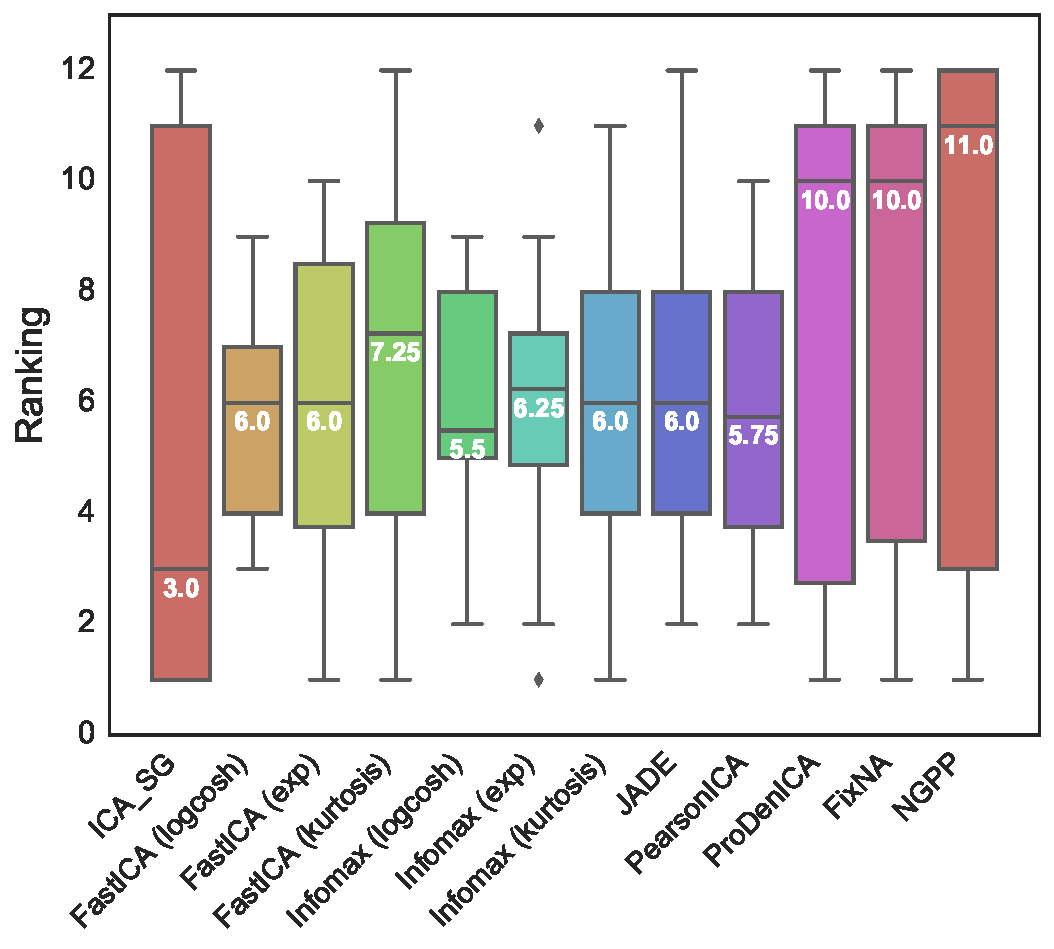
\includegraphics[width=2.2in]{ranking/images_boxplot-r2.pdf}
}\\
\end{center}
\caption{Results of ICA methods in the case of mixture of images and noise. \textbf{Moze nie powtarzac, jest juz w subcaptions to samo}}
\label{fig:rank1}
\end{figure*}

%\begin{landscape}
\begin{figure*}[t]
% ensure that we have normalsize text
\normalsize
\begin{center}
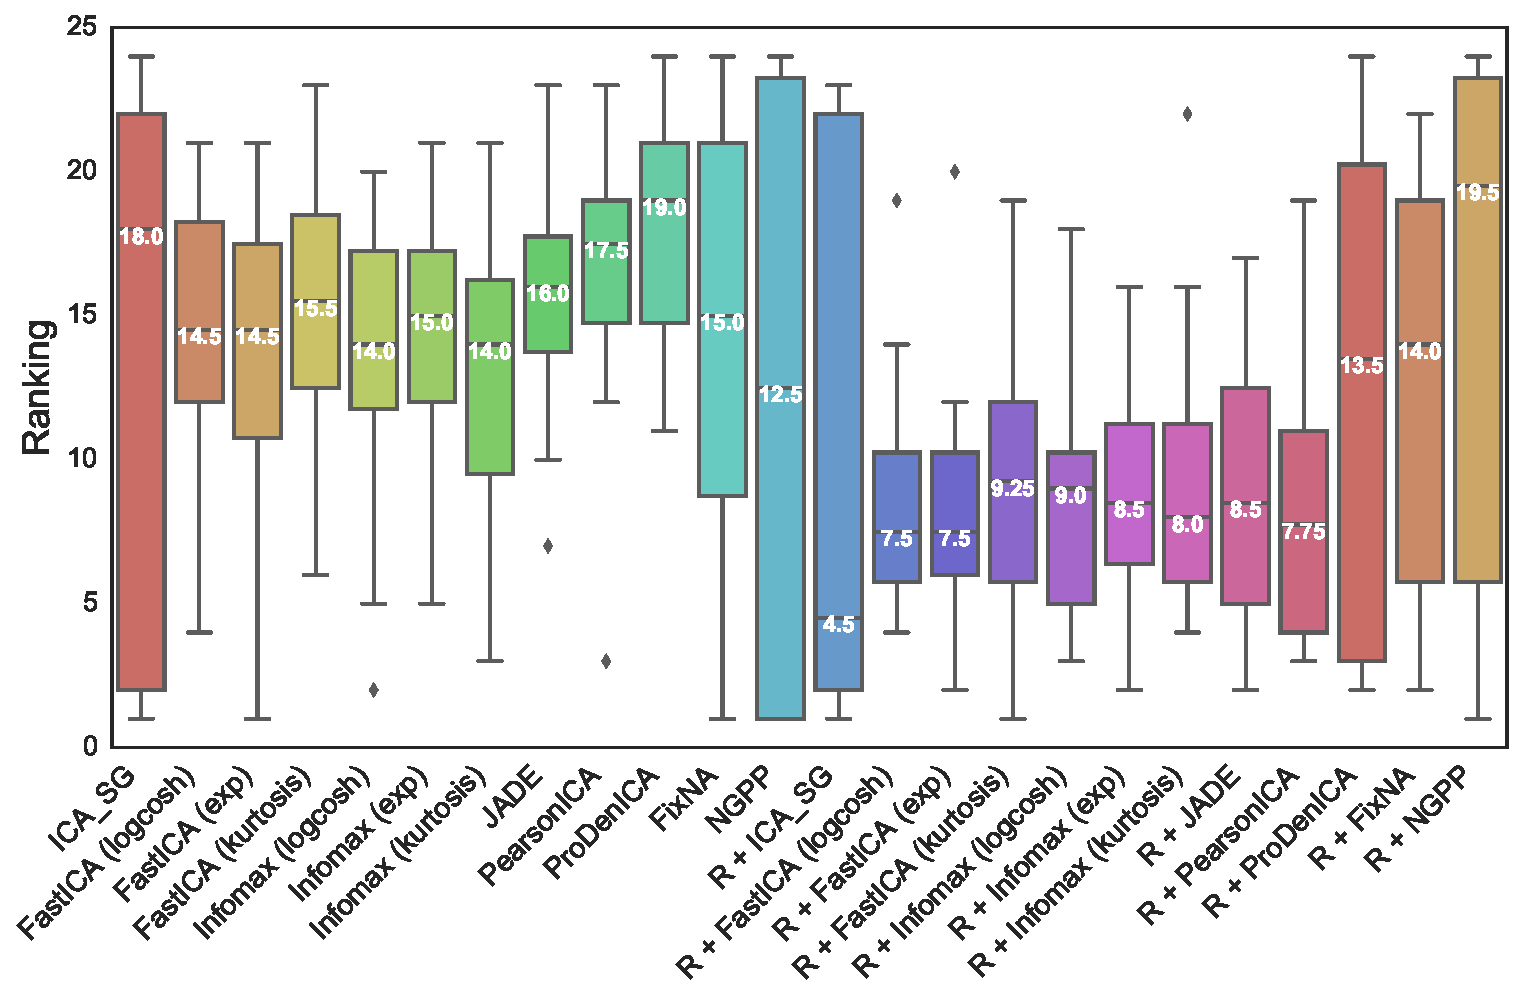
\includegraphics[width=4.0in]{ranking/images_boxplot-r3.pdf}
\end{center}
\caption{Results of ICA methods in the case of mixture of images and noise salt and pepper noise with scale (R+) and without preprocessing.}
\label{fig:rank2}
\end{figure*}

To compare \ICA{} to other state-of-the-art approaches we use 
Tucker's congruence coefficient \cite{lorenzo2006tucker} which values range between $-1$ and $+1$. It can be used to study the similarity of extracted factors across different samples. Generally, a congruence coefficient of $0.9$ indicates a high degree of factor similarity, while a coefficient of $0.95$ or higher indicates that the factors are virtually identical. 

We evaluate our method in the context of 2D and hyperspectral images. 
For comparison we use R package {\tt ica} \cite{ica}, {\tt PearsonICA} \cite{pearsonica}, {\tt ProDenICA} \cite{prodenica}, {\tt tsBSS} \cite{tsBSS}, {\tt NGPP} \cite{virta2016projection}.
The most popular method used in practice is FastICA \cite{hyvarinen1999fast,helwig2013critique} algorithm, which uses negentropy. In this context we can use three different functions to estimate neg-entropy:
logcosh, exp and kurtosis.
We also compare our method with algorithm using Information-Maximization (Infomax) approach \cite{bell1995information}. Similarly to FastICA we consider three possible non-linear functions: hyperbolic tangent, logistic and extended Infomax.
%We also consider algorithm which uses Joint Approximate Diagonalization of Eigenmatrices (JADE) proposed by Cardoso and Souloumiac's \cite{cardoso1993blind,helwig2013critique}.
%
%One of the most popular ICA methods dedicated for skew data is PearsonICA \cite{karvanen2000pearson,karvanen2002blind}, which minimizes mutual information using a Pearson \cite{stuart1968advanced} system-based parametric model. Another model we consider is ProDenICA \cite{bach2002kernel,hastie2009elements}, which is based not on a
%single nonlinear function, but on an entire function space of candidate nonlinearities. In particular, the method works with the functions in a reproducing kernel Hilbert space, and make use of the “kernel trick” to search over this space efficiently. 
%We also compare our method with  FixNA \cite{shi2009blind}, method for blind source separation problem.
%

%\begin{landscape}
\begin{figure*}[t]
% ensure that we have normalsize text
\normalsize
\begin{center}
  \subfigure[Original images 42049 and 220075 and Gaussian nice \textbf{noise}.] {\label{fig:image_ICA_res_1}
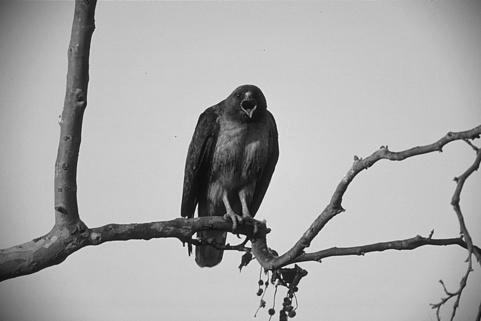
\includegraphics[width=1.4in]{3/2_6_or_1} 
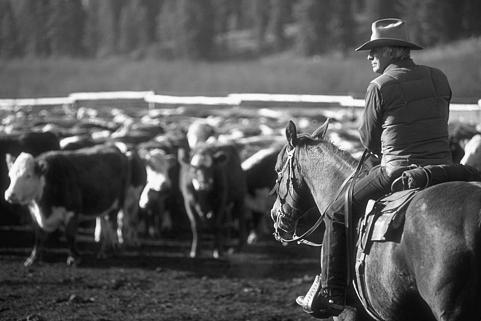
\includegraphics[width=1.4in]{3/2_6_or_2}

\includegraphics[width=1.4in]{3/2_6_or_3}
}
%\subfigure[Mixture of sources.] {\label{fig:image_ICA_res_1}
%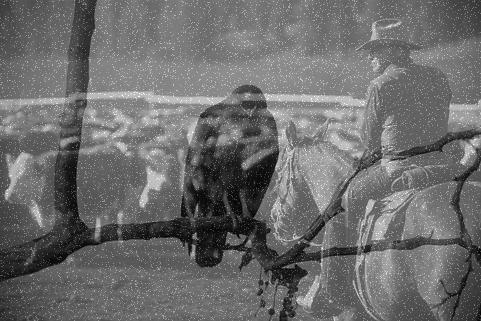
\includegraphics[width=0.9in]{3/2_6_div_1} 
%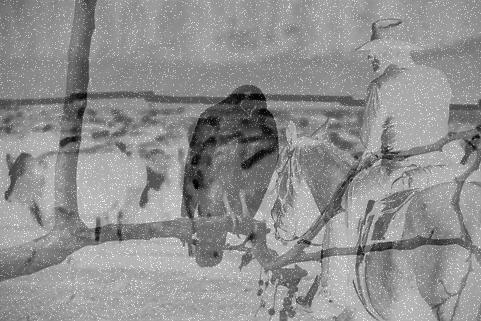
\includegraphics[width=0.9in]{3/2_6_div_2}
%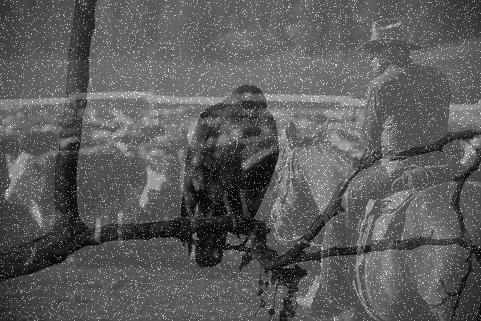
\includegraphics[width=0.9in]{3/2_6_div_3}
%}
\subfigure[Mixture of sources after rescaling.] {\label{fig:image_ICA_res_1}
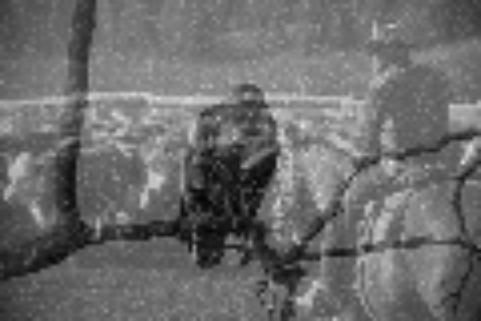
\includegraphics[width=1.4in]{3/2_6_div_1_r} 
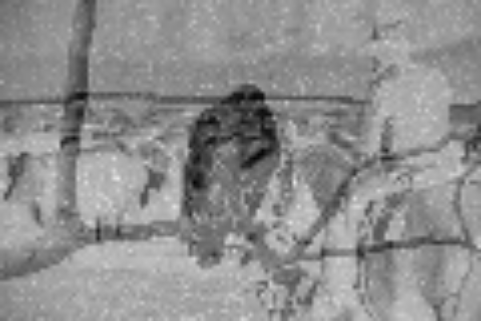
\includegraphics[width=1.4in]{3/2_6_div_2_r}
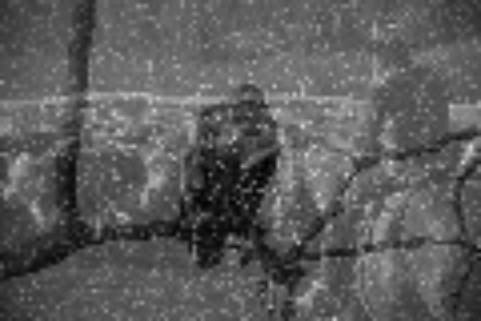
\includegraphics[width=1.4in]{3/2_6_div_3_r}
}

%%%%%%%%%%%%%%%%%%%%
%\subfigure[Sum and subtraction of images.] {\label{fig:image_ICA_int_2}
%\includegraphics[width=1.2in]{2/2_6_sum} 
%\includegraphics[width=1.2in]{2/2_6_div}
%} \\

%%%%%%%%%%%%%%%%%%%%
\subfigure[\ICA.] {\label{fig:image_ICA_res_3}
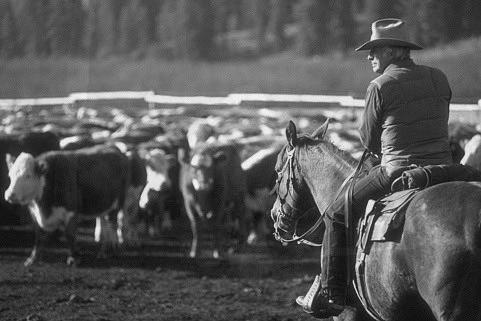
\includegraphics[width=1.in]{3/2_6_SGD_2} 
}
\subfigure[FastICA.] {\label{fig:image_ICA_res_4}
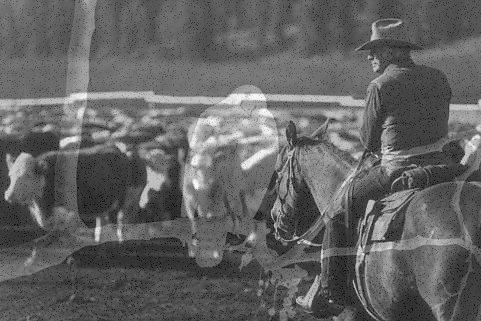
\includegraphics[width=1.in]{3/2_6_ICA11_2} 
}
\subfigure[ProDenICA.] {\label{fig:image_ICA_res_5}
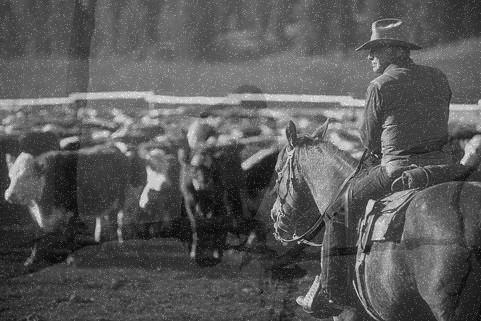
\includegraphics[width=1.in]{3/2_6_ICA5_2} 
}
\subfigure[NGPP.] {\label{fig:image_ICA_res_9}

\includegraphics[width=1.in]{3/2_6_ICA8_1}
}\\
%%%%%%%%%%%%%%%%%%%%

\subfigure[\ICA.] {\label{fig:image_ICA_res_6}
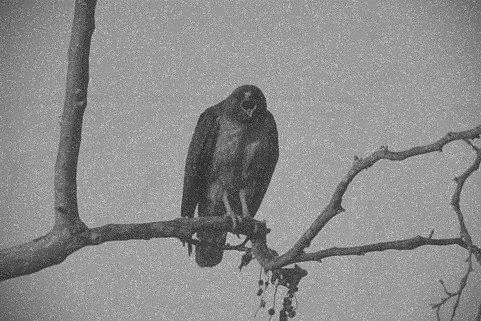
\includegraphics[width=1.in]{3/2_6_SGD_1}
}
\subfigure[FastICA.] {\label{fig:image_ICA_res_7}
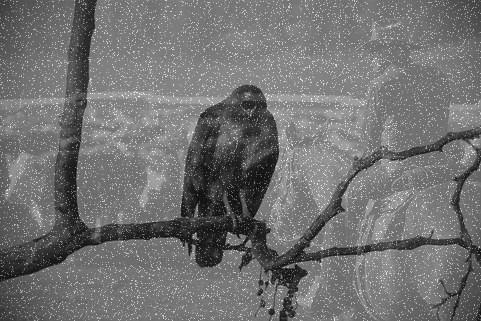
\includegraphics[width=1.in]{3/2_6_ICA11_1}
}
\subfigure[ProDenICA.] {\label{fig:image_ICA_res_8}
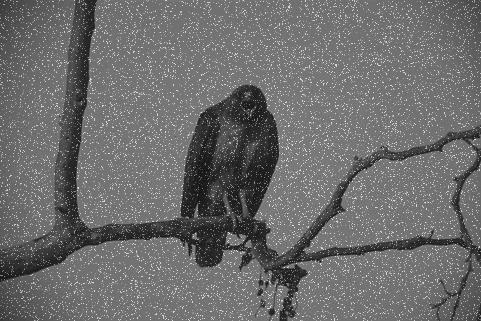
\includegraphics[width=1.in]{3/2_6_ICA5_1}
}
\subfigure[NGPP.] {\label{fig:image_ICA_res_10}
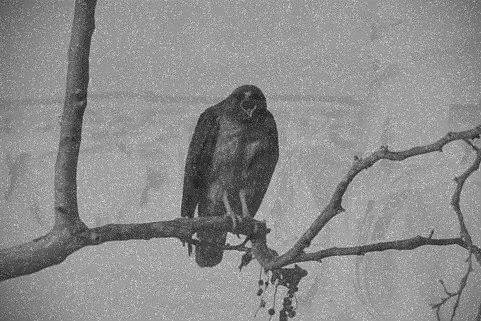
\includegraphics[width=1.in]{3/2_6_ICA8_2}
}
\end{center}
\caption{Comparison of images separation by our method (\ICA), with FastICA,  ProDenICA, NGPP. \textbf{Ale to jest to samo co Fig.1 -- po co powtarzac?} }
\label{fig:image_ICA_res}
\end{figure*}


\subsection{Separation of images}

One of the most popular application of ICA is the separation of images. In our experiments we use four images from the USC-SIPI Image Database of size $256 \times 256$ pixels (4.1.01, 4.1.06, 4.1.02, 4.1.03) and eight of size $512 \times 512$ pixels (4.2.04, 4.2.02, boat.512, elaine.512, 5.2.10, 5.2.08, 5.3.01, 4.2.03). We also use 8 images from the Berkeley Segmentation Dataset of size $482 \times 321$ with indexes (\#119082, \#42049, \#43074, \#38092, \#157055, \#220075, \#295087, \#167062). 

We make random pairs of above images and one component with noise (random sample from Gaussian distribution $\nor(0,1)$) and use them as a source signal combined by the mixing matrix $A = \begin{bmatrix} 1 & 1 & 1  \\ 1 & -1 & -1 \\ -1 & 1 & -1  \end{bmatrix} $. Our goal was to reconstruct two original images by using only the knowledge about mixed ones. The visualization of this process we present in Fig. \ref{fig:image_ICA_int}. 

\begin{table*}[t]
\label{tab:congru_img_1}
\vskip 0.15in
\begin{center}
\begin{small}
\begin{sc}
\resizebox{\textwidth}{!}{
\begin{tabular}{ c | c c c c c c c c  c  c  c  c c}
\hline
%\abovespace\belowspace
 & \ICA  & FastICA & FastICA & FastICA & Infomax & Infomax & Infomax & JADE & PearsonICA & ProDenICA & \ \  FixNA & \ \ NGPP\\ 
  &  &  logcosh & exp & kurtosis & tanh & tangent & logistic &  & & & & \\
\hline
%\abovespace
Source 1 & 0.3427 & 0.2778 & 0.2820 & 0.2865 & 0.2823 & 0.2731 & 0.2979 & 0.2901 & 0.2837 & 0.2065 & 0.1827 & 0.1820 \\
Source 2 & 0.3212 & 0.4122 & 0.3954 & 0.3690 & 0.4168 & 0.4193 & 0.1972 & 0.3611 & 0.2679 & 0.1318 & 0.3020 & 0.3176 \\
Source 3 & 0.3180 & 0.1857 & 0.1878 & 0.1285 & 0.1845 & 0.1819 & 0.3782 & 0.0053 & 0.0252 & 0.2565 & 0.0426 & 0.2962 \\
Source 4 & 0.2822 & 0.0357 & 0.0364 & 0.1743 & 0.0339 & 0.0208 & 0.0317 & 0.1780 & 0.2802 & 0.1724 & 0.3196 & 0.1768 \\

\hline
\end{tabular}
}
\end{sc}
\end{small}
\end{center}
\caption{Tucker's congruence coefficients between average edges form reference layers and various ICA results.}
\end{table*}

As a summary from the experiment, in Figure \ref{fig:rank1_a} we present a boxplot \textbf{czy miales na mysli box plots?} of \textbf{the} ranks obtained by the methods.
The \ICA {} almost perfectly recovered source signal and it is one of the best in ranking. 
Although this is not surprising as the experiments were in fact conducted in the setting which favored our approach, as we chose the noise to be gaussian, \textbf{Znowu sie kajamy, czy potrzebnie to spytaj Jacka. Ale jakos niezgrabnie?} this shows that \ICA{} works as desired and deals well with removing \textbf{any} gaussian components from the data. 

In the next experiments we reaped \textbf{repeated?} the procedure with salt and pepper \textbf{``salt and pepper''} noise. But \textbf{usun But} before applying ICA methods we rescale images, see Fig. \ref{fig:image_ICA_res}. 
Such procedure can be understand as a preprocessing in the ICA framework. After rescaling of images non-gaussian noise become more normal and therefore we are able to remove them. In Figure \ref{fig:rank1_a} we present a boxplot \textbf{box plot? box plots? box-plot?} of ranks obtained on rescale data \textbf{on the rescaled data}. 

The rescaling of images give sensational \textbf{lepiej vastly zamiast sensational} better results in the case of non-gaussian noise end increase \textbf{and increases the} score of all methods, see Figure \ref{fig:rank2}. 


%\begin{landscape}
\begin{figure*}[t!]
% ensure that we have normalsize text
\normalsize
\begin{center}
%\subfigure[The effect of the \ICA \ method.] {\label{fig:image_1}
%  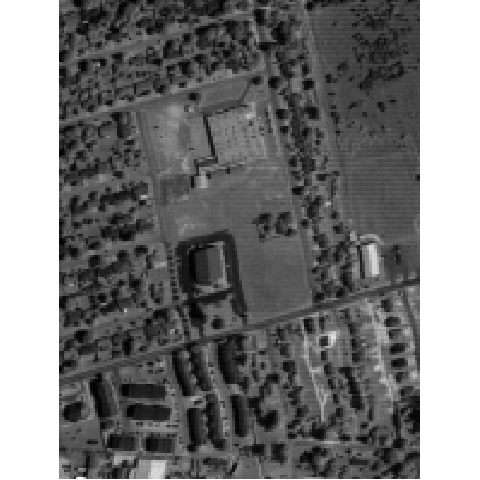
\includegraphics[width=1.2in]{spec/1a} 
%  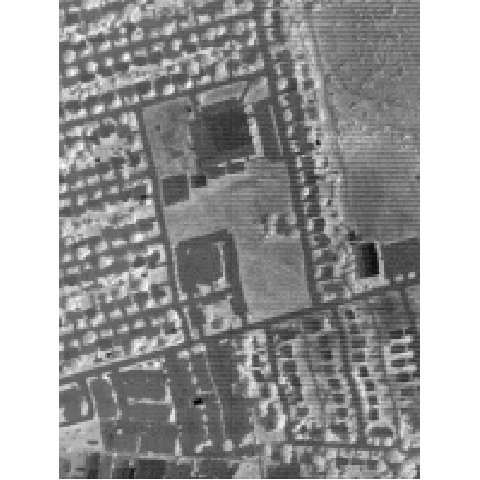
\includegraphics[width=1.2in]{spec/2a}
%  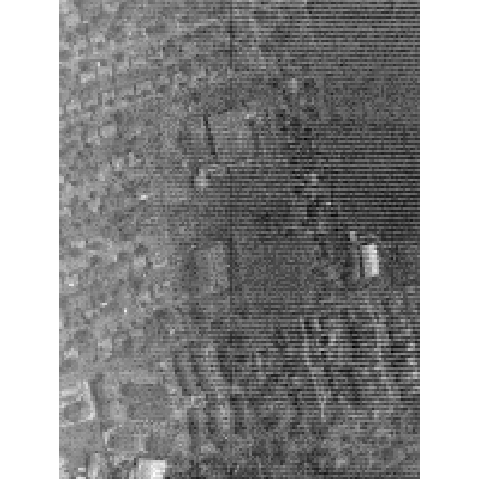
\includegraphics[width=1.2in]{spec/3a} 
%  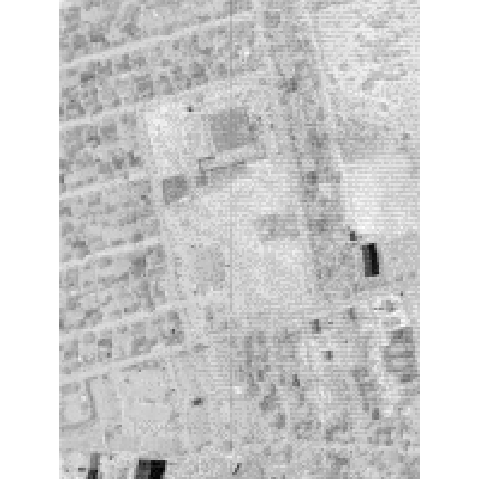
\includegraphics[width=1.2in]{spec/4a}
%} \\
%%%%%%%%%%%%%%%%%%%%%%%%%%%%%%%%%%
%%%%%%%%%%%%%%%%%%%%%%%%%%%%%%%%%%
\subfigure[Ground truth layers which contains 4 channels: \#1 Asphalt, \#2 Grass, \#3 Tree and \#4 Roof.] {\label{fig:image_1}
  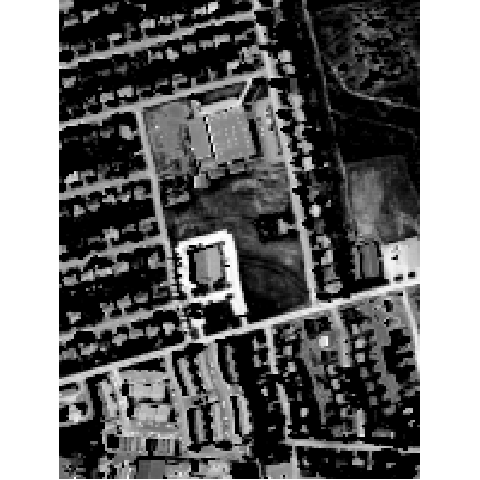
\includegraphics[width=1.in]{spec/O_1} 
  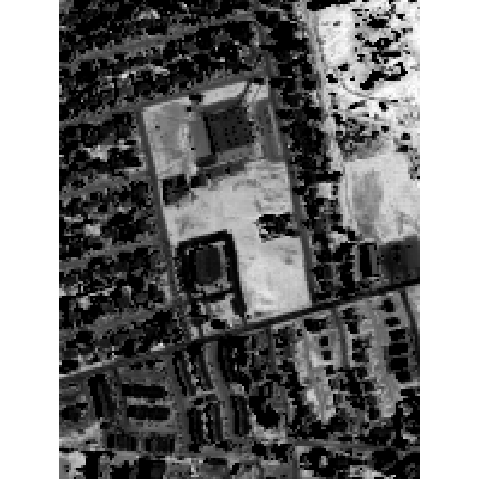
\includegraphics[width=1.in]{spec/O_2}
  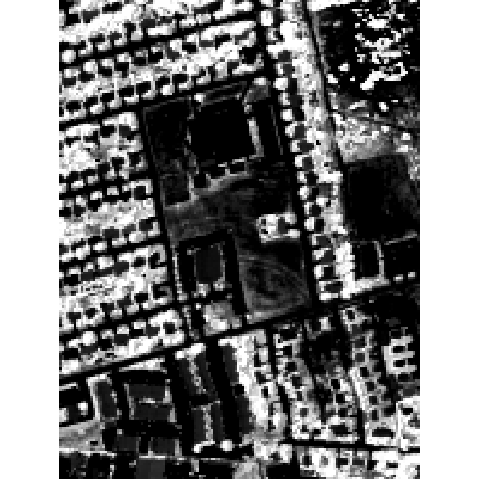
\includegraphics[width=1.in]{spec/O_3} 
  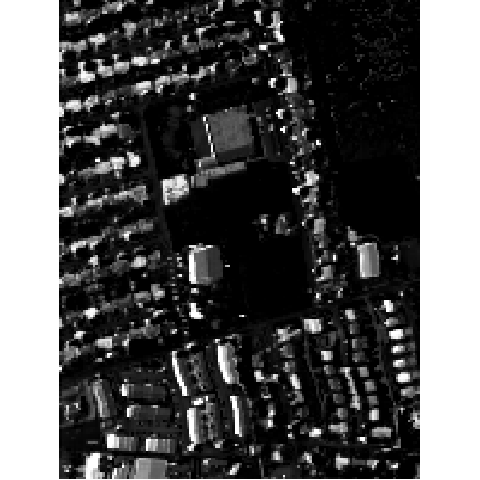
\includegraphics[width=1.in]{spec/O_4}
} \\
%%%%%%%%%%%%%%%%%%%%%%%%%%%%%%%%%%
%%%%%%%%%%%%%%%%%%%%%%%%%%%%%%%%%%
\subfigure[The effect of the \ICA \ method.] {\label{fig:image_2}
  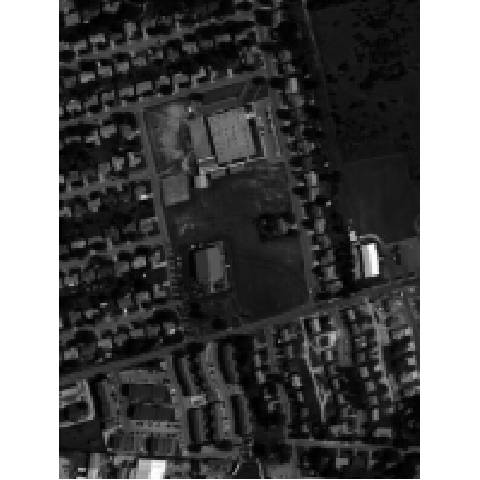
\includegraphics[width=1.in]{spec/SG_1} 
  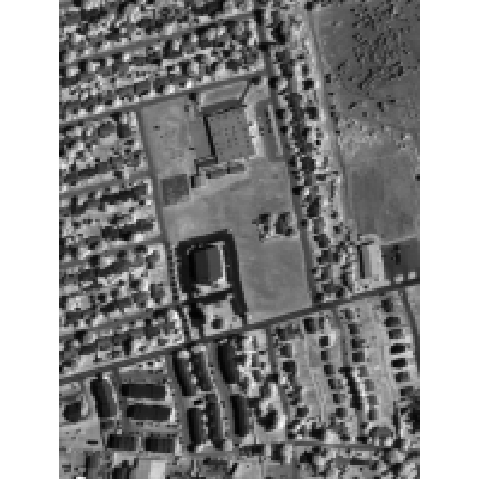
\includegraphics[width=1.in]{spec/SG_2}
  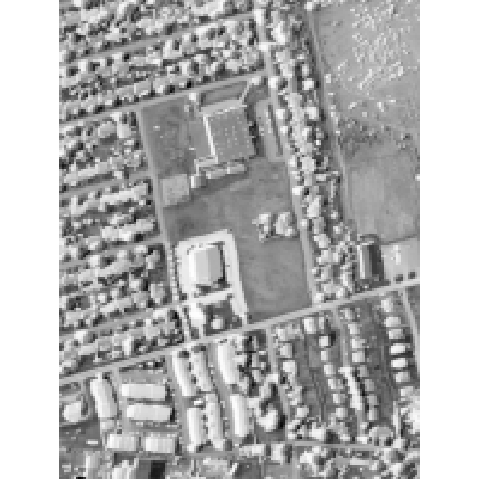
\includegraphics[width=1.in]{spec/SG_3} 
  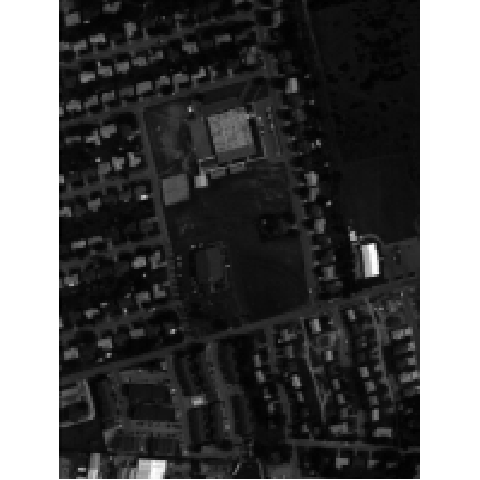
\includegraphics[width=1.in]{spec/SG_4}
} \\
%%%%%%%%%%%%%%%%%%%%%%%%%%%%%%%%%%
%%%%%%%%%%%%%%%%%%%%%%%%%%%%%%%%%%
\subfigure[The effect of the FastICA (logcosh) method.] {\label{fig:image_3}
  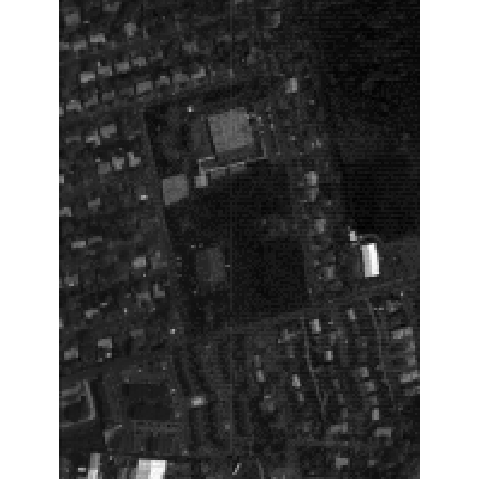
\includegraphics[width=1.in]{spec/ICA11_3} 
  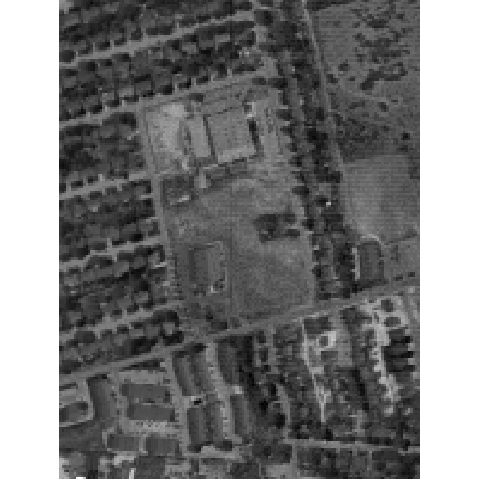
\includegraphics[width=1.in]{spec/ICA11_2}
  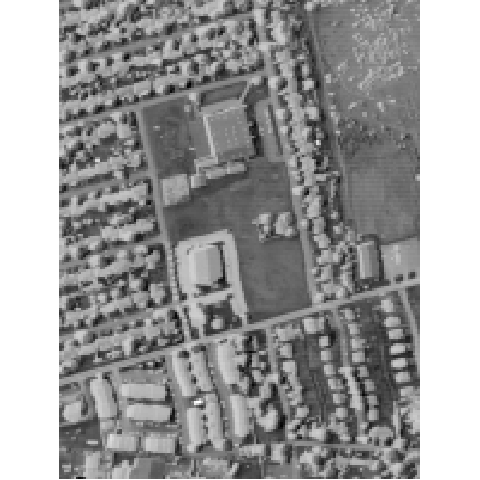
\includegraphics[width=1.in]{spec/ICA11_1} 
  
\includegraphics[width=1.in]{spec/ICA11_4}
} \\
%%%%%%%%%%%%%%%%%%%%%%%%%%%%%%%%%%
%%%%%%%%%%%%%%%%%%%%%%%%%%%%%%%%%%
%\subfigure[The effect of the PearsonICA method.] {\label{fig:image_1}
%  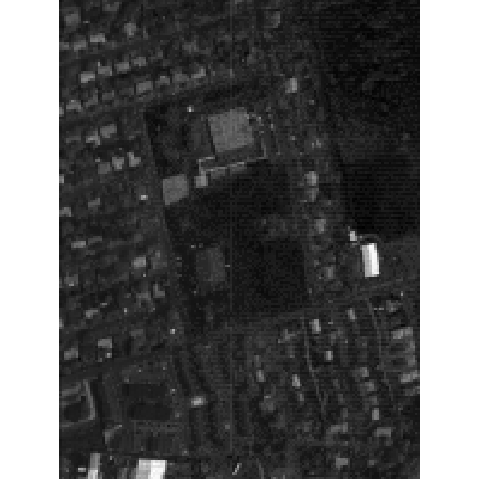
\includegraphics[width=1.2in]{spec/ica_41} 
%  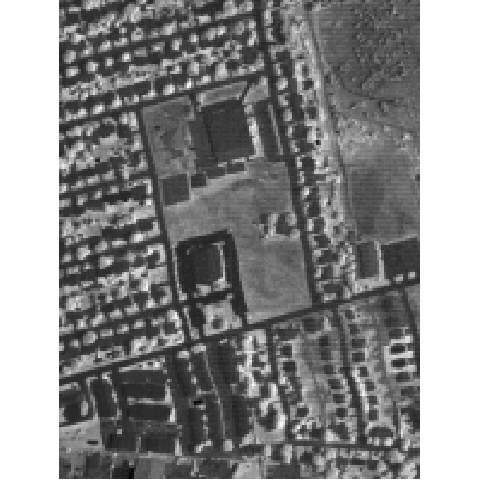
\includegraphics[width=1.2in]{spec/ica_42}
%  \includegraphics[width=1.2in]{spec/ica_43} 
%  \includegraphics[width=1.2in]{spec/ica_44}
%} \\
%%%%%%%%%%%%%%%%%%%%%%%%%%%%%%%%%%
%%%%%%%%%%%%%%%%%%%%%%%%%%%%%%%%%%
\subfigure[The effect of the  ProDenICA method.] {\label{fig:image_4}
  \includegraphics[width=1.in]{spec/ICA5_1} 
  \includegraphics[width=1.in]{spec/ICA5_4}
  \includegraphics[width=1.in]{spec/ICA5_3} 
  \includegraphics[width=1.in]{spec/ICA5_2}
} \\
%%%%%%%%%%%%%%%%%%%%%%%%%%%%%%%%%%
%%%%%%%%%%%%%%%%%%%%%%%%%%%%%%%%%%
\subfigure[The effect of the  NGPP method.] {\label{fig:image_5}
  \includegraphics[width=1.in]{spec/ICA8_1} 
  \includegraphics[width=1.in]{spec/ICA8_2}
  \includegraphics[width=1.in]{spec/ICA8_3} 
  \includegraphics[width=1.in]{spec/ICA8_4}
} 
\end{center}
\caption{Results of image separation with the uses of various ICA algorithms.}
\label{fig:spec_1}
\end{figure*}


\subsection{Hyperspectral Unmixing}

Independent component analysis has been recently \textbf{can be zamiast has been recently?}
applied into \textbf{to zamiast into} hyperspectral unmixing 
\cite{wang2015abundance}
as a result of \textbf{lepiej due to} its low
computation time and its ability to perform without prior information.
In this subsection we apply \textbf{present a zamiast apply} simple example which suggests that our method also can by used for spectral data.

Urban data  \cite{fyzhu2014IJPRSSSNMF,fyzhu2014TIPDgSNMF,fyzhu2014JSTSPRRLbSF} is one of the most widely used hyperspectral data-sets used \textbf{usun used} in the hyperspectral \textbf{usun hyperspectral} unmixing study. Each image has $307 \times 307$ pixels, each of which corresponds to a $2 \times 2$ m area. In this image, there are 210 wavelengths ranging from 400 nm  to 2500 nm, resulting in a spectral resolution of 10 nm. After the channels 1--4, 76, 87, 101--111, 136--153 and 198--210 are removed (due to dense water vapor and atmospheric effects), there remain 162  channels (this is a common preprocess for hyperspectral unmixing analyses). There is ground truth \cite{fyzhu2014IJPRSSSNMF,fyzhu2014TIPDgSNMF,fyzhu2014JSTSPRRLbSF}, which contains 4 channels: \#1 Asphalt, \#2 Grass, \#3 Tree and \#4 Roof.

A highly mixed area is cut from the original data set in this experiment (similar example was showed in \cite{wang2015abundance}), with the size of $200 \times 150$ pixels. %Fig. \ref{} shows the true-color image. 

In our experiment we compared \ICA{} to other popular ICA methods, see Fig. \ref{fig:spec_1}. Observe that \ICA{}, NGPP and ProDenICA give layers which seem to contain more information then FastICA, as the last component in FastICA contains mainly noise. To verify which method separate sources from noise better we calculate how obtained layers corresponds to original signals. Since there is no classical measure for such task \textbf{przecinek} we verified it by calculation \textbf{calculating the} correlation coefficient between \textbf{the} average muse \textbf{co to jest muse? moze literowka a moze ja nie znam slowa} of edges of reference layers (in our experiment we use Canny edge detector \textbf{zrob z tego osobne zdanie}) and ICA results, see Tab. \ref{tab:congru_img_1}. Our method gives similar \textbf{comparable zamiast similar} value of similarity measure on all layers. 


%
%\begin{table*}[t]
%\caption{Classification accuracies for naive Bayes and flexible 
%Bayes on various data sets.}
%\label{tab:congru_img_1}
%\vskip 0.15in
%\begin{center}
%\begin{small}
%\begin{sc}
%\resizebox{\textwidth}{!}{
%\begin{tabular}{ c c c c c c c c c  c  c  c  c }
%\hline
%%\abovespace\belowspace
% & \ICA  & FastICA & FastICA & FastICA & Infomax & Infomax & Infomax & JADE & PearsonICA & ProDenICA \\ 
%  &  &  logcosh & exp & kurtosis & tanh & tangent & logistic &  & &  \\
%\hline
%%\abovespace
%
%\hline
%\end{tabular}
%}
%\end{sc}
%\end{small}
%\end{center}
%\vskip -0.1in
%\end{table*}

%\begin{table*}[!t]
%\centering
%\scalebox{0.7}{ 
%\begin{tabular}{ | c | c  | c c c | c c c | c | c | }
%\multicolumn{1}{c}{} & \multicolumn{1}{c}{\ICA}  & \multicolumn{3}{c}{FastICA} & \multicolumn{3}{c}{Infomax}  & \multicolumn{1}{c}{PearsonICA} & \multicolumn{1}{c}{ProDenICA}  \\ 
% &  &  logcosh & exp & kurtosis & tanh & tangent & logistic & &  \\
%\hline
%\#1 Asphalt  &\bf 0.6774 &  0.2859 & 0.2864 & -0.2595 & -0.2972 & -0.2954 &  -0.2972 &  0.20978 & 0.4928  \\
%\#2 Grass  & \bf -0.7784 &  -0.2746 & -0.2605 &  -0.2798 &  -0.2814 & -0.2816 & -0.2814 &  -0.2412 & -0.4323  \\
%\#3 Tree  & \bf 0.7267 & 0.2338 &  0.2717 &  -0.2547 &  0.2441 & 0.2354 &  0.2442 &   0.2482 & -0.5961  \\
%\#4 Roof &\bf 0.6666 &  -0.4256 &  0.4279 &  0.4167 & -0.4244 &  0.4301 & -0.4244 &  0.4193 &  -0.6128  \\
%
%\end{tabular}
%}
%\caption{The Tucker's congruence coefficient measure between reference layers and results of different ICA algorithms in the case of the urban data set.}
%\label{tab:spec}
%\end{table*}


%\begin{figure*}[!t]
%\normalsize
%\begin{center}
%\includegraphics[width=5in]{spec_1}
%\end{center}
%\caption{Congruence distance between layers obtain by different ICA algorithms and the closest reference channel.}
%\label{fig:spec_1}
%\end{figure*}





%%%%%%%%%%%%%%%%%%%%%%%%%%%%%%%%

    
%%%%%%%%%%%%%%%%%%%%%%%%%%%%%%%%
\section{Appendix A}
\label{a1}
%%%%%%%%%%%%%%%%%%%%%%%%%%%%%%%%%%%%%%%%%%%%%%%%%%%%%%%%%%%%%%%%
\begin{proof}[Proof of Theorem \ref{the:min}.]
\textbf{Zrob tak zeby sie proof nie powtarzal 2x w naglowku w tym i innych twierdzeniach w appendixie}
Let $X=\{ \x_1, \ldots, \x_n \}$.
We write 
\begin{equation*}
\z_i= W(\x_i-m), \quad \z_{ij}= \w_j^T(\x_i-m),
\end{equation*}
for observation $i$, where $i=1,\ldots,n$ and coordinates $j=1,\ldots,d$.

Let us consider the likelihood function, i.e. 
$$
\begin{array}{l}
L(X;\m,W,\sigma,\tau) = \prod\limits_{i=1}^{n} SN_{d}N_{D-d}(\x_i; \m,W, \sigma^2,\tau^2) \\[6pt] 
=\prod\limits_{i=1}^{n} | \det(W)|  \prod\limits_{j=1}^{d} SN(  \w_j^T (\x_i - \m) ; 0 , \sigma_j^2, \tau_j^2) \cdot %\\[6pt]
\prod\limits_{j=d+1}^{D} N(  \w_j^T (\x_i - \m) ; 0 , \sigma_j^2) =\\[6pt]
\Big( c_1|\det(W)| \Big)^{n} 
\Big( \prod\limits_{j=1}^{d} \sigma_j(1+\tau_j) \Big)^{-n} %\cdot \\[6pt]
\prod\limits_{i=1}^{n} %\\[6pt]
\prod\limits_{j=1}^{d} \exp \Big[ -\frac{1}{2\sigma_j^2}z_{ij}^2 (\1_{ \{ z_{ij} \leq 0 \} } + %\\[6pt]
\tau_{j}^{-2} \1_{ \{ z_{ij} > 0 \} }) \Big] \\[6pt]
\Big( \prod\limits_{j=d+1}^{D} \sigma_j \Big)^{-n} \prod\limits_{i=1}^{n}\prod\limits_{j=d+1}^{D} \exp \Big[ -\frac{1}{2\sigma_j^2}z_{ij}^2 \Big],
\end{array}
$$
%$$
%\begin{array}{l}
%= \prod\limits_{i=1}^{n} GSN_d(\x_i ; \m,V,\sigma,\tau)
%= \prod\limits_{i=1}^{n} \frac{1}{| \det( V)|}  \prod\limits_{j=1}^{d} SN(  \v^{-1}_j \x_i ; \v^{-1}_j \m , \sigma_j^2, \tau_j^2)=
%\\[1ex]
%\left(\frac{c_1}{|\det(V)|}\right)^{n} \left( \prod\limits_{j=1}^{d} \sigma_j(1+\tau_j) \right)^{-n} \left( \prod\limits_{i=1}^{n} \prod\limits_{j=1}^{d} \exp[-\frac{1}{2\sigma_j^2}z_{ij}^2 (\1_{ \{ z_{ij} \leq 0 \} } + \tau_{j}^{-2} \1_{ \{ z_{ij} > 0 \} })]\right)
%\end{array}
%$$
where 
$
c_1= \left( \sqrt{\tfrac{2}{\pi}} \right)^{d} \cdot \left( \tfrac{1}{ \sqrt{2\pi} } \right)^{D-d}.
$
Now we take the log-likelihood function, i.e. 
$$
\begin{array}{l}
\ln(L(X;\m,W,\sigma,\tau)) = \ln \bigg( \Big( c_1|\det(W)| \Big)^{n} \Big( \prod\limits_{j=1}^{d} \sigma_j(1+\tau_j) \Big)^{-n} \Big( \prod\limits_{j=d+1}^{D} \sigma_j \Big)^{-n}  \bigg) + \\[6pt]
 \sum\limits_{i=1}^{n} \sum\limits_{j=1}^{d} \Big[ -\frac{1}{2\sigma_j^2}z_{ij}^2 (\1_{ \{ z_{ij} \leq 0 \} } + \tau_{j}^{-2} \1_{ \{ z_{ij} > 0 \} })\Big] +  %\\[6pt]
 \sum\limits_{i=1}^{n} \sum\limits_{j=d+1}^{D} \Big[ -\frac{1}{2\sigma_j^2}z_{ij}^2 \Big]  \\[6pt]
= \ln \bigg( \Big( c_1|\det(W)| \Big)^{n} \Big( \prod\limits_{j=1}^{d} (1+\tau_j) \Big)^{-n} \Big( \prod\limits_{j=1}^{D} \sigma_j \Big)^{-n} \bigg)  - \\[6pt]
  \frac{1}{2} \sum\limits_{j=1}^{d} \Big( \sigma_j^{-2} \sum\limits_{i \in I_{j}}    z_{ij}^2   + \frac{\sigma_j^{-2}}{\tau_{j}^{2} }  \sum\limits_{i \in I_{j}^{c}}   z_{ij}^2  \Big) -  %\\[6pt]
  \frac{1}{2} \sum\limits_{j=d+1}^{D} \sigma_j^{-2} \Big( \sum\limits_{i \in I_{j}}    z_{ij}^2   +  \sum\limits_{i \in I_{j}^{c}}   z_{ij}^2  \Big) \\[6pt]
= \ln \bigg( \Big( c_1|\det(W)| \Big)^{n} \Big( \prod\limits_{j=1}^{d} (1+\tau_j) \Big)^{-n} \Big( \prod\limits_{j=1}^{D} \sigma_j \Big)^{-n} \bigg) - \\[6pt]
 \sum\limits_{j=1}^{d} \frac{1}{2\sigma_j^{2}} \Big(  s_{1j}  + \frac{1}{\tau_{j}^{2} }  s_{2j}  \Big) - \sum\limits_{j=d+1}^{D} \frac{1}{2\sigma_j^{2}} \Big(  s_{1j}  + s_{2j}  \Big).
\end{array}
$$

We fix  $\m$, $W$ and maximize the log-likelihood function over $\tau$ and $\sigma$.
In such a case \textbf{zamiast In such a case uzyj Consequently} we have to \textbf{zamiast we have to uzyj we need to} solve the following system of equations
$$
\begin{array}{l}
\frac{\partial  \ln ( L(X;\m,W,\sigma,\tau) ) }{\partial \sigma_j} =0, \qquad %\\[6pt] & \mbox{ for }  & j=1,\ldots,d,
 \frac{\partial  \ln ( L(X;\m,W,\sigma,\tau) ) }{\partial \tau_j} =0 , %& \mbox{ for }  & j=1,\ldots,d.
\end{array}
$$
for  $ j=1,\ldots,D$. Hence \textbf{It follows that zamiast Hence}
$$
\begin{array}{l}
-\frac{n}{\sigma_j} +  \sigma_j^{-3} (s_{1j} + \tau_j^{-2} s_{2j} ) = 0, \mbox{ for }  j=1,\ldots,d,\\[6pt]
 -\frac{n}{\sigma_j} +  \sigma_j^{-3} (s_{1j} + s_{2j} ) =0, \mbox{ for } j>d, \\[6pt] %
- \frac{n}{1+\tau_j} + \frac{s_{2j}}{\tau_j^{3}\sigma_j^{2}} =0 , \mbox{ for } j=1,\ldots,d.
\end{array}
$$
By simple calculations we obtain the expressions for the estimators in \ref{eq:est}.
%\begin{align*}
%$$
%\hat{\sigma}_j^2(\m,W) = 
%\tfrac{1}{n} s_{1j}^{2/3} g_{j}(\m,W), \qquad
%\hat{\tau}_{j}(\m,W) = \bigg( \frac{s_{2j}}{s_{1j}} \bigg)^{1/3}.
%$$
%\end{align*}
Substituting it into the log-likelihood function,
%and taking $e^{\ln \hat{L}(\m,W)}$
we get %$$
$$
\begin{array}{l}
\hat{L}(\m,W) = \bigg( \frac{2}{\pi} \bigg)^{\frac{dn}{2}}  \bigg( \frac{1}{2\pi} \bigg)^{\frac{(D-d)n}{2}} \!\!\!\!\! |\det(W)|^{n} \Big( \prod\limits_{j=1}^{d} \frac{1}{\sqrt{n}} g_j(\m,W)^{\frac{3}{2}} \Big)^{-n} \!\!\!\!\!
e^{-\frac{dn}{2}} \Big( \prod\limits_{j=d+1}^{D} (\frac{s_{1j} + s_{2j}}{n})^{\frac{1}{2}} \Big)^{-n} \!\!\!\!\! = \\[6pt]
\frac{ 2^{(d-D/2)n} n^{dn/2} }{(\pi e)^{Dn/2}} \cdot %\\[6pt]
\Big( \frac{1}{|\det(W)|^{\frac{2}{3}}} \prod\limits_{j=1}^{d} g_j(\m,W) \Big)^{-\frac{3n}{2}} \Big( \prod\limits_{j=d+1}^{D} \frac{(s_{1j} + s_{2j})}{n} \Big)^{-\frac{n}{2}} 
\end{array}
$$
%= \bigg( \frac{2n}{\pi e} \bigg)^{\frac{dn}{2}} =
\end{proof}

%%%%%%%%%%%%%%%%%%%%%%%%%%%%%%%%


%%%%%%%%%%%%%%%%%%%%%%%%%%%%%%%%
%%%%%%%%%%%%%%%%%%%%%%%%%%%%%%%%
\section{Appendix B}
\label{a2}
%%%%%%%%%%%%%%%%%%%%%%%%%%%%%%%%

We will need the following well-known lemma (for the convenience of the reader we provide the proof).

\begin{lemma}\label{jacobi}
%\comment{Jacek mowi, ze powino być A(t), i napisać co to znaczy adj()}
Let $A = (a_{ij})_{1 \leq i,j \leq d}$ be a differentiable map from real numbers to $d \times d$ matrices then
\begin{equation}
\frac{\partial \det(A)}{\partial a_{ij}} = \mathrm{adj}^T(A)_{ij},
\end{equation}
where $\mathrm{adj}(A)$ stands for the adjugate of $A$, i.e. the transpose of the cofactor matrix.
\end{lemma}

\begin{proof}
By the Laplace expansion $\det A = \sum\limits_{j=1}^{d} (-1)^{i+j} a_{ij} M_{ij}$ where $M_{ij}$ is the minor of the entry in the $i$-th row and $j$-th column. Hence
$$\frac{\partial \det A}{\partial a_{ij}} = (-1)^{i+j} M_{ij} = \mathrm{adj}^T(A)_{ij}.$$
\end{proof}

\begin{proof}[Proof of Theorem \ref{ther:grad}.]
Let us start with the partial derivative of $\ln({l})$ with respect to $\m$. We have
$$
\begin{array}{l}
\frac{\partial \ln {l}(X;\m,W)}{\partial \m_k} =
\sum \limits_{j=1}^d \frac{\partial \ln ({g}_j(\m,W))}{\partial \m_k} + \sum \limits_{j=d+1}^D \frac{\partial \ln ((s_{1j}+s_{2j})^{\frac{1}{3}})}{\partial \m_k} \\[6pt]
= \sum\limits_{j=1}^d \frac{1}{{s}_{1j}^{\frac{1}{3}} + {s}_{2j}^{\frac{1}{3}}} \frac{\partial ({s}_{1j}^{\frac{1}{3}} + {s}_{2j}^{\frac{1}{3}})}{\partial \m_k} + \sum\limits_{j=d+1}^D \frac{1}{({s}_{1j} + {s}_{2j})^{\frac{1}{3}}} \frac{\partial (({s}_{1j} + {s}_{2j})^{\frac{1}{3}})}{\partial \m_k} \\[6pt]
= \sum \limits_{j=1}^d \frac{1}{{s}_{1j}^{\frac{1}{3}} + {s}_{2j}^{\frac{1}{3}}} \bigg(
\frac{1}{3 {s}_{1j}^{\frac{2}{3}}} \frac{\partial {s}_{1j}}{\partial \m_k} +
\frac{1}{3 {s}_{2j}^{\frac{2}{3}}} \frac{\partial {s}_{2j}}{\partial \m_k}
\bigg) \\[6pt]
+ \sum \limits_{j=d+1}^D \frac{1}{({s}_{1j} + {s}_{2j})^{\frac{1}{3}}} \frac{1}{3} \frac{1}{({s}_{1j} + {s}_{2j})^{\frac{2}{3}}}\bigg(
\frac{\partial {s}_{1j}}{\partial \m_k} +
\frac{\partial {s}_{2j}}{\partial \m_k}
\bigg).
\end{array}
$$
Now, we need $\frac{\partial {s}_{1j}}{\partial \m_k}$ and $\frac{\partial {s}_{2j}}{\partial \m_k}$, therefore
$$
\begin{array}{l}
\frac{\partial {s}_{1j}}{\partial \m_k} = 
\sum\limits_{i \in {I}_j} \frac{\partial [\w^T_j (\x_i - \m)]^2}{\partial \m_k} =\\[6pt]
 \sum\limits_{i \in {I}_j} 2 \w^T_j (\x_i - \m) \frac{\partial \w^T_j (\x_i - \m)}{\partial \m_k} = %\\[6pt]
 \sum\limits_{i \in {I}_j} - 2 \w^T_j (\x_i - \m) \w_{jk}.
\end{array}
$$
Analogously we get
$$
\begin{array}{l}
\frac{\partial {s}_{2j}}{\partial \m_k} = \sum\limits_{i \in {I}_j^c} -2 \w^T_j (\x_i - \m) \w_{jk}.
\end{array}
$$
%\comment{$\v^{-1}_{jk} = \w_{jk}$}\\
Hence 
$$
\begin{array}{l}
\frac{\partial \ln {l}}{\partial \m_k} =\sum\limits_{j=1}^d \frac{-1}{{s}_{1j}^{\frac{1}{3}} + {s}_{2j}^{\frac{1}{3}}} \bigg(
\frac{1}{3 {s}_{1j}^{\frac{2}{3}}} \sum\limits_{i \in I_j} 2 \w_j^T (\x_i - \m)  \w_{jk} + \\[6pt]
\frac{1}{3 {s}_{2j}^{\frac{2}{3}}} \sum\limits_{i \in I_j^c} 2 \w_j^T (\x_i - \m) \w_{jk}
\bigg) + \sum\limits_{j=d+1}^D \frac{-1}{3(s_{1j}+s_{2j})} \cdot \\[6pt]
\bigg(
 \sum\limits_{i \in I_j} 2 \w_j^T (\x_i - \m)  \w_{jk} +% \\[6pt]
 \sum\limits_{i \in I_j^c} 2 \w_j^T (\x_i - \m) \w_{jk}
\bigg)
.
\end{array}
$$

Now we calculate the partial derivative of $\ln {l}(X;\m,W)$ with respect to the matrix $W$. We have $\frac{\partial \ln {l}(X;\m,W)}{\partial \w_{pk}} =$
$$
\begin{array}{l}
\frac{\partial \ln |\det(W)|^{-\frac{2}{3}}}{\partial \w_{pk}} + \sum\limits_{j=1}^d \frac{\partial \ln ({g}_j(\m,W))}{\partial \w_{pk}}
+ \sum\limits_{j=d+1}^D \frac{\partial \ln ( (s_{1j}+s_{2j})^{\frac{1}{3}} )}{\partial \w_{pk}}.
\end{array}
$$
%\comment{$\v_{pk}^{-1} = \w_{pk}$}\\
To calculate the derivative of the determinant we use Jacobi's formula (see Lemma \ref{jacobi}).
Hence% $\frac{\partial \ln (\det(W)^{-\frac{2}{3}})}{\partial \w_{pk}} =$
$$
\begin{array}{l}
\frac{\partial \ln (\det(W)^{-\frac{2}{3}})}{\partial \w_{pk}} = \det(W)^{\frac{2}{3}}  \Big(-\frac{2}{3}\Big)  \det(W)^{-\frac{5}{3}}  \frac{\partial \det(W)}{\partial \w_{pk}} \\[6pt]
= -\frac{2}{3} \det(W)^{-1}  \mathrm{adj}^T(W)_{pk} \\[6pt]
 = -\frac{2}{3} \frac{1}{\det(W)}  \left[\det(W)  (W^{-1})^T_{pk}\right]= -\frac{2}{3}  (\w^{-1})^T_{pk},
\end{array}
$$
where $(\w^{-1})^T_{pk}$ is the element in the $p$-th row and $k$-th column of the matrix $(W^{-1})^T$. Now we calculate %$\frac{\partial \ln ({g}_j(\m,W))}{\partial \w_{pk}} =$
$$
\begin{array}{l}
\frac{\partial \ln ({g}_j(\m,W))}{\partial \w_{pk}} = \frac{1}{{s}_{1j}^{\frac{1}{3}} + {s}_{2j}^{\frac{1}{3}}} \frac{\partial ({s}_{1j}^{\frac{1}{3}} + {s}_{2j}^{\frac{1}{3}})}{\partial \w_{pk}}= \\[6pt]
\frac{1}{{s}_{1j}^{\frac{1}{3}} + {s}_{2j}^{\frac{1}{3}}} \bigg(
\frac{1}{3 {s}_{1j}^{\frac{2}{3}}}  \frac{\partial {s}_{1j}}{\partial \w_{pk}} +
\frac{1}{3 {s}_{2j}^{\frac{2}{3}}}  \frac{\partial {s}_{2j}}{\partial \w_{pk}}
\bigg),
\end{array}
$$
where
$$
\begin{array}{l}
\frac{\partial {s}_{1j}}{\partial \w_{pk}} = \sum\limits_{ i \in {I}_j} \frac{\partial [\w^T_j (\x_i - \m)]^2}{\partial \w_{pk}} = \sum\limits_{ i \in {I}_j} 2 \w^T_j (\x_i - \m) \frac{\partial \w^T_j (\x_i - \m)}{\partial \w_{pk}}
\\[6pt]
= \left\{ \begin{array}{ll}
0, & \text{if} \; j\neq p\\
\sum\limits_{ i \in {I}_p} 2 \w^T_p (\x_i - \m) (\x_{ik} - \m_k), & \text{if} \; j=p\\
\end{array} \right.
\end{array}
$$
and $\x_{ik}$ is the $k$-th element of the vector $\x_i$. Analogously we get
$$\frac{\partial {s}_{2j}}{\partial \w_{pk}} = \left\{ \begin{array}{ll}
0, & \text{if} \; j\neq p\\
\sum\limits_{ i \in {I}_p^c} 2 \w^T_p (\x_i - \m) (\x_{ik} - \m_k), & \text{if} \; j=p.
\end{array} \right.
$$
Moreover,
$$
\begin{array}{l}
\frac{\partial \ln ( (s_{1j}+s_{2j})^{\frac{1}{3}} )}{\partial \w_{pk}} = \frac{1}{ (s_{1j}+s_{2j})^{\frac{1}{3}} } \frac{\partial ( (s_{1j}+s_{2j})^{\frac{1}{3}} )}{\partial \w_{pk}}= \\[6pt]
\frac{1}{ (s_{1j}+s_{2j})^{\frac{1}{3}} } \frac{1}{3} \frac{1}{ (s_{1j}+s_{2j})^{\frac{2}{3}} } \bigg(
  \frac{\partial {s}_{1j}}{\partial \w_{pk}} +
  \frac{\partial {s}_{2j}}{\partial \w_{pk}}
\bigg),
\end{array}
$$
Hence we obtain
$$
\begin{array}{l}
\frac{\partial \ln {l}}{\partial \w_{pk}} = -\frac{2}{3} (\w^{-1})^T_{pk} + \\[6pt]
\frac{1}{{s}_{1p}^{\frac{1}{3}} +{s}_{2p}^{\frac{1}{3}}} 
 \bigg(
\frac{1}{3} {s}_{1p}^{-\frac{2}{3}} \sum\limits_{ i \in {I}_p} 2 \w^T_p (\x_i - \m) (\x_{ik} - \m_k)\\[6pt]
+ \frac{1}{3} {s}_{2p}^{-\frac{2}{3}} \sum\limits_{ i \in {I}_p^c} 2 \w^T_p (\x_i - \m) (\x_{ik} - \m_k) \bigg)+\\[6pt]

\frac{1}{ 3(s_{1p}+s_{2p}) } 
 \bigg(
\sum\limits_{ i \in {I}_p} 2 \w^T_p (\x_i - \m) (\x_{ik} - \m_k) + \\[6pt]
\sum\limits_{ i \in {I}_p^c} 2 \w^T_p (\x_i - \m) (\x_{ik} - \m_k) \bigg)
.
\end{array}
$$

\end{proof}
%%%%%%%%%%%%%%%%%%%%%%%%%%%%%%%%


\bibliography{ref}
\bibliographystyle{plain}

%\paragraph{Remark 1.}
%\begin{equation}
%  \psi (u) = \int_{o}^{T} \left[\frac{1}{2}
%  \left(\Lambda_{o}^{-1} u,u\right) + N^{\ast} (-u)\right] dt \;  .
%\end{equation}

%\medskip
%\noindent
%{\it Example of a Computer Program}
%\begin{verbatim}
%program Inflation (Output)
%  {Assuming annual inflation rates of 7%, 8%, and 10%,...
%   years};
%   const
%     MaxYears = 10;
%   var
%     Year: 0..MaxYears;
%     Factor1, Factor2, Factor3: Real;
%   begin
%     Year := 0;
%     Factor1 := 1.0; Factor2 := 1.0; Factor3 := 1.0;
%     WriteLn('Year  7% 8% 10%'); WriteLn;
%     repeat
%       Year := Year + 1;
%       Factor1 := Factor1 * 1.07;
%       Factor2 := Factor2 * 1.08;
%       Factor3 := Factor3 * 1.10;
%       WriteLn(Year:5,Factor1:7:3,Factor2:7:3,Factor3:7:3)
%     until Year = MaxYears
%end.
%\end{verbatim}
%%
%\noindent
%{\small (Example from Jensen K., Wirth N. (1991) Pascal user manual and
%report. Springer, New York)}


%\begin{thebibliography}{4}
%
%\bibitem{jour} Smith, T.F., Waterman, M.S.: Identification of Common Molecular
%Subsequences. J. Mol. Biol. 147, 195--197 (1981)
%
%\bibitem{lncschap} May, P., Ehrlich, H.C., Steinke, T.: ZIB Structure Prediction Pipeline:
%Composing a Complex Biological Workflow through Web Services. In: Nagel,
%W.E., Walter, W.V., Lehner, W. (eds.) Euro-Par 2006. LNCS, vol. 4128,
%pp. 1148--1158. Springer, Heidelberg (2006)
%
%\bibitem{book} Foster, I., Kesselman, C.: The Grid: Blueprint for a New Computing
%Infrastructure. Morgan Kaufmann, San Francisco (1999)
%
%\bibitem{proceeding1} Czajkowski, K., Fitzgerald, S., Foster, I., Kesselman, C.: Grid
%Information Services for Distributed Resource Sharing. In: 10th IEEE
%International Symposium on High Performance Distributed Computing, pp.
%181--184. IEEE Press, New York (2001)
%
%\bibitem{proceeding2} Foster, I., Kesselman, C., Nick, J., Tuecke, S.: The Physiology of the--
%Grid: an Open Grid Services Architecture for Distributed Systems
%Integration. Technical report, Global Grid Forum (2002)
%
%\bibitem{url} National Center for Biotechnology Information, \url{http://www.ncbi.nlm.nih.gov}
%
%\end{thebibliography}
%

%\section*{Appendix: Springer-Author Discount}

%LNCS authors are entitled to a 33.3\% discount off all Springer
%publications. Before placing an order, the author should send an email, 
%giving full details of his or her Springer publication,
%to \url{orders-HD-individuals@springer.com} to obtain a so-called token. This token is a
%number, which must be entered when placing an order via the Internet, in
%order to obtain the discount.
%
%\section{Checklist of Items to be Sent to Volume Editors}
%Here is a checklist of everything the volume editor requires from you:
%
%
%\begin{itemize}
%\settowidth{\leftmargin}{{\Large$\square$}}\advance\leftmargin\labelsep
%\itemsep8pt\relax
%\renewcommand\labelitemi{{\lower1.5pt\hbox{\Large$\square$}}}
%
%\item The final \LaTeX{} source files
%\item A final PDF file
%\item A copyright form, signed by one author on behalf of all of the
%authors of the paper.
%\item A readme giving the name and email address of the
%corresponding author.
%\end{itemize}
\end{document}
